\documentclass[12pt]{beamer}

% for themes, etc.
\mode<presentation>
{ \usetheme{default} }

\usepackage{graphicx}        % standard LaTeX graphics tool
                             % when including figure files
\usepackage{multicol}        % used for the two-column index
\usepackage[bottom]{footmisc}% places footnotes at page bottom

\usepackage{enumerate,verbatim}
\usepackage{amssymb,amsmath,ulem}
\usepackage{transparent}
\usepackage{tikz}
\usepackage{algpseudocode}

\newcommand{\D}{\mathrm{d}}
\newcommand{\subt}[1]{\framesubtitle{#1}}
\newcommand{\dst}{\displaystyle}
\newcommand{\spa}{\vspace{0.5cm}\newline}

\setbeamertemplate{itemize item}{$\circ$}

\usefonttheme{professionalfonts}

\setbeamertemplate{navigation symbols}{}
\setbeamertemplate{footline}{\hfill \small \insertframenumber/\inserttotalframenumber \vspace{0.1in} \hspace{0.025in}   }%/ }


\setbeamercolor{title}{fg=black}
\setbeamercolor{frametitle}{fg=black}

\setbeamertemplate{frametitle}{\insertframetitle\\\usebeamerfont{framesubtitle}\insertframesubtitle}
%\setbeamerfont{frametitle}{size=\scriptsize}
\setbeamerfont{framesubtitle}{size=\normalsize}




\title{Notes on B{\'e}zier Shapes}
\author{\textbf{Daniel W. Zaide}\\ dan.zaide@gmail.com}
\institute{Scientific Computation Research Center, Rensselaer Polytechnic Institute}
\date{February 26, 2016}


\AtBeginSection[]
{
  \begin{frame}
    \frametitle{Table of Contents}
    \tableofcontents[currentsection]
  \end{frame}
}
\begin{document}
%%%%%%%%%% TITLE SLIDE
\begin{frame}[plain]
\titlepage
\end{frame}
\begin{frame}
\frametitle{Table of Contents}
\tableofcontents[]
\end{frame}
\section{Introduction to B{\'e}zier Shapes}
\begin{frame}{B{\'e}zier shapes}
$P^{th}$ order B{\'e}zier shapes can be defined as follows:
{
  \scriptsize

\begin{eqnarray*}
\mathrm{Edge} & \mathbf{B}(u)& = \displaystyle \sum_{i+j=P} \frac{P!}{i!j!}u^iv^j\mathbf{C}_{ij}, \quad v = 1-u\\
\mathrm{Triangle} & \mathbf{B}(u,v)& = \displaystyle\sum_{i+j+k=P} \frac{P!}{i!j!k!}u^iv^jw^k\mathbf{C}_{ijk}, \quad w = 1-u-v
\\
\mathrm{Tet} & \mathbf{B}(u,v,w)& = \displaystyle\sum_{i+j+k+l=P} \frac{P!}{i!j!k!l!}u^iv^jw^kt^l\mathbf{C}_{ijkl}, \quad t = 1-u-v-w
\end{eqnarray*}
}
With all parameters as barycentric coordinates, \[u,v,w,t \in [0,1] \]
There is often the use of the binomial coefficient, here I will also use that notation, with
{
  \scriptsize

\[ \frac{P!}{i!j!} = {P \choose i},\qquad \frac{P!}{i!j!k!} = {P \choose i,j},\qquad \frac{P!}{i!j!k!l!} = {P \choose i,j,k}\]
\[\frac{P!}{i!j!k!} = {P \choose i}{P-i \choose j},\qquad \frac{P!}{i!j!k!l!} = {P \choose i}{P-i \choose j}{P-i-j \choose k}\]
}
\end{frame}
\begin{frame}{B{\'e}zier Triangle}
For example, the $4^{th}$ order B{\'e}zier Triangle is drawn here, to illustrate the control points and notation.
\begin{figure}
\centering
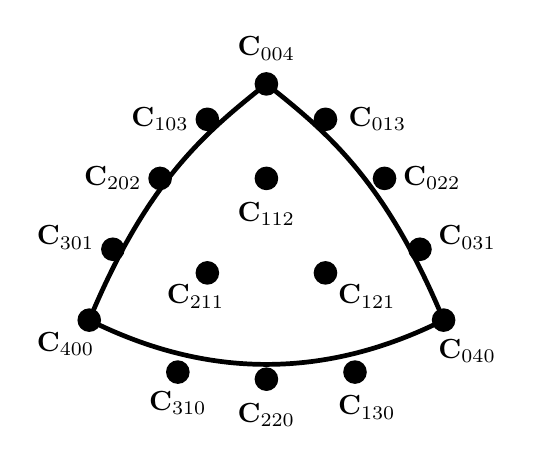
\begin{tikzpicture}[scale=3.0] 
\draw [line width=0.6mm, black ] (0, 0) .. controls (0.5,-0.25) and (1.0, -0.25)
   .. (1.5, 0.) .. controls (1.25,0.6) and (1.0,0.8) 
   .. (0.75,1.) .. controls (0.5,0.8) and (0.25,0.6) 
   .. (0,0); 

\path (-0.1,-0.1) node {$\mathbf{C}_{400}$}
(0.375,-0.35) node {$\mathbf{C}_{310}$}
(0.75,-0.4) node {$\mathbf{C}_{220}$}
(1.175,-0.37) node {$\mathbf{C}_{130}$}
(1.6,-0.13) node {$\mathbf{C}_{040}$}
(1.6,0.35) node {$\mathbf{C}_{031}$}
(1.45,0.6) node {$\mathbf{C}_{022}$}
(1.22,0.85) node {$\mathbf{C}_{013}$}
(0.75,1.15) node {$\mathbf{C}_{004}$}
(-0.1,0.35) node {$\mathbf{C}_{301}$}
(0.1,0.6) node {$\mathbf{C}_{202}$}
(0.3,0.85) node {$\mathbf{C}_{103}$}
(0.45,0.1) node {$\mathbf{C}_{211}$}
(1.175,0.1) node {$\mathbf{C}_{121}$}
(0.75,0.45) node {$\mathbf{C}_{112}$};
\fill (0,0) circle [radius=0.5mm];
\fill (0.375,-0.22) circle [radius=0.5mm];
\fill (.75,-.25) circle [radius=0.5mm];
\fill (1.125,-.22) circle [radius=0.5mm];
\fill (1.5,0) circle [radius=0.5mm];
\fill (1.4,0.3) circle [radius=0.5mm];
\fill (1.25,0.6) circle [radius=0.5mm];
\fill (1.0,0.85) circle [radius=0.5mm];
\fill (0.1,0.3) circle [radius=0.5mm];
\fill (0.3,0.6) circle [radius=0.5mm];
\fill (0.5,0.85) circle [radius=0.5mm];
\fill (0.5,0.2) circle [radius=0.5mm];
\fill (1.0,0.2) circle [radius=0.5mm];
\fill (0.75,0.6) circle [radius=0.5mm];
\fill (0.75,1.) circle [radius=0.5mm];
\end{tikzpicture}
\end{figure}
\end{frame}
\begin{frame}{Number of Control Points}
For $P^{th}$ order B{\'e}zier shapes contain the following number of control points

\begin{tabular}{l|cccc}
 & Total & Internal\\ \hline
Curve & $P+1$ & $P-1$ \\
Triangle & $\frac{1}{2}(P+1)(P+2)$ & $\frac{1}{2}(P-1)(P-2)$ \\
Tet & $\frac{1}{6}(P+1)(P+2)(P+3)$ &$\frac{1}{6}(P-1)(P-2)(P-3)$\\

\end{tabular}\spa
For example,\spa
\begin{tabular}{l|cccc}
Order & Tri Total & Tri Internal & Tet Total & Tet Internal\\ \hline
4 & 15 & 3 & 35 & 1\\
5 & 21 & 6 & 56 & 4\\
6 & 28 & 10 & 84 & 10
\end{tabular}
\end{frame}
\begin{frame}{Useful Properties}
\begin{itemize}
 \item The convex hull property. The max and min values of a B\'{e}zier polynomial evaluated within the domain are bounded by the max and min values of its corresponding control points.
 \item Variation diminishing. The curve has no more intersections with any plane than polygon of its control points, and converges to the curve.
 \item Affine invariance. Curves form an affine map, allowing for reparametrization. 
 \item Degree elevation and subdivision. Curves can be increased to higher-orders without changing behavior of the curve.
 \item Derivatives of B{\'e}zier  shapes are themselves B{\'e}zier shapes.
 \item Edges of B{\'e}zier triangles are B{\'e}zier curves and faces of B{\'e}zier tets are B{\'e}zier triangles.
\end{itemize}

\end{frame}
\begin{frame}{Convex Hull Property}
The Convex Hull property of B{\'e}zier shapes guarantees that the shape will lie entirely inside its convex hull. The curve below is inside the hull formed by its control points.
\begin{figure}
\centering
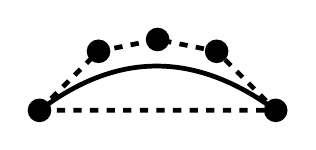
\begin{tikzpicture}[scale=3.0] 
\draw [line width=0.6mm, black ] (0, 0) .. controls (0.33,0.25) and (0.66,0.25)
   .. (1.0, 0.);
\fill (0,0) circle [radius=0.5mm];
\fill (0.25,0.25) circle [radius=0.5mm];
\fill (0.5,0.3) circle [radius=0.5mm];
\fill (.75,.25) circle [radius=0.5mm];
\fill (1.,0) circle [radius=0.5mm];
\draw [line width=0.6mm, black,dashed ] (0,0) -- (0.25,0.25) -- (0.5,0.3) -- (.75,.25) -- (1.,0) -- (0,0);
\end{tikzpicture}
\end{figure}
This property guarantees a bound on the shape based solely on its control points, and is important in the validity calculations.
\end{frame}
\section{Elevation}
\begin{frame}{Elevation}
Elevation is the property of B{\'e}zier shapes that describes increasing the order of the shape without changing it. Elevating a curve by one order is shown below
\begin{figure}
\centering
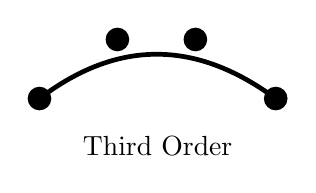
\begin{tikzpicture}[scale=3.0] 
\draw [line width=0.6mm, black ] (0, 0) .. controls (0.33,0.25) and (0.66,0.25)
   .. (1.0, 0.);
\fill (0,0) circle [radius=0.5mm];
\fill (0.33,0.25) circle [radius=0.5mm];
\fill (.66,.25) circle [radius=0.5mm];
\fill (1.,0) circle [radius=0.5mm];
\node at (0.5,-0.2) {Third Order};
\end{tikzpicture}
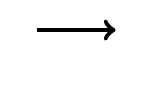
\begin{tikzpicture}
\draw[line width=0.6mm,->] (0,0.5) -- (1.0,0.5);
\node at (0,0) {};
\end{tikzpicture}
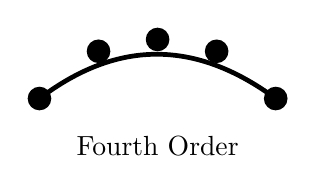
\begin{tikzpicture}[scale=3.0] 
\draw [line width=0.6mm, black ] (0, 0) .. controls (0.33,0.25) and (0.66,0.25) .. (1.0, 0.);
\fill (0,0) circle [radius=0.5mm];
\fill (0.25,0.2) circle [radius=0.5mm];
\fill (0.5,0.25) circle [radius=0.5mm];
\fill (.75,.2) circle [radius=0.5mm];
\fill (1.,0) circle [radius=0.5mm];
\node at (0.5,-0.2) {Fourth Order};
\end{tikzpicture}
\end{figure}
We note that as we elevate the curve, the control points converge to the shape itself.
\end{frame}
\begin{frame}{Elevation - Curves}
To elevate an order $P$ curve by one order, we have
\[ \mathbf{C}^{P+1}_i = \frac{i}{P+1}\mathbf{C}^P_{i-1} + \left(1-\frac{i}{P+1}\right)\mathbf{C}^P_i, \quad 1 \leq i \leq P\]
Generalized to elevate by $r$ orders, we get 
\[
\mathbf{C}^{P+r}_i = \displaystyle \sum_{j = \max(0,i-r)}^{\min(i,P)} \frac{{P \choose i}{r \choose i-j}}{{P+r \choose i}}\mathbf{C}^P_j, \quad 1 \leq i < P+r
\]

\end{frame}
\begin{frame}{Elevation - Triangles}
Elevating triangles is achieved similarly. To elevate by $r$ orders, we have that
\[ \mathbf{C}^{P+r}_{ij} = \displaystyle\sum_{k = \max(0,i-r)}^{\min(i,P)}\sum_{l = \max(0,i-k+j-r)}^{\min(j,P-k)} 
\frac{{P \choose k,l}{r \choose i-k,j-l}}{{P+r \choose i,j}}\mathbf{C}^P_{lk} \]
with $i+j=P+r$. In practice, we could elevate the edges separately from the internal points, however this is not currently done.
\end{frame}
\section{Subdivision}
\begin{frame}{Subdivision}
Subdividing a B{\'e}zier shape splits it it into multiple shapes that together exactly represent the original shape. Curves become two curves, and triangles become three triangles. For a third order curve subdivided at $u = 1/2$, we get the diagram below

\begin{figure}
\centering
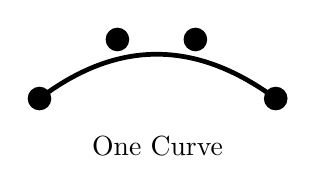
\begin{tikzpicture}[scale=3.0] 
\draw [line width=0.6mm, black ] (0, 0) .. controls (0.33,0.25) and (0.66,0.25)
   .. (1.0, 0.);
\fill (0,0) circle [radius=0.5mm];
\fill (0.33,0.25) circle [radius=0.5mm];
\fill (.66,.25) circle [radius=0.5mm];
\fill (1.,0) circle [radius=0.5mm];
\node at (0.5,-0.2) {One Curve};
\end{tikzpicture}
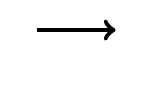
\begin{tikzpicture}
\draw[line width=0.6mm,->] (0,0.5) -- (1.0,0.5);
\node at (0,0) {};
\end{tikzpicture}
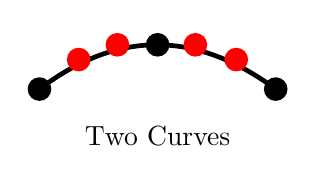
\begin{tikzpicture}[scale=3.0] 
\draw [line width=0.6mm, black ] (0, 0) .. controls (0.33,0.25) and (0.66,0.25) .. (1.0, 0.);
\fill (0,0) circle [radius=0.5mm];
\fill[fill=red] (0.166,0.125) circle [radius=0.5mm];
\fill[fill=red] (0.33,0.1875) circle [radius=0.5mm];
\fill (0.5,0.1875) circle [radius=0.5mm];
\fill[fill=red] (0.66,0.1875) circle [radius=0.5mm];
\fill[fill=red] (0.833,0.125) circle [radius=0.5mm];
\fill (1.,0) circle [radius=0.5mm];
\node at (0.5,-0.2) {Two Curves};
\end{tikzpicture}
\end{figure}
Again, the new control points all converge to the actual curve.
\end{frame}
\begin{frame}{Subdivision - Curves}
Subdivision is fairly straight forward, computed using de Casteljau's algorithm. We note that we can write any curve as a sum of two curves of one degree lower,
{
  \scriptsize

\begin{eqnarray*} \mathbf{B}(u) &=& \sum_{i=0}^P {P \choose i} u^i(1-u)^{P-i}\mathbf{C}_{i} \\ &=& (1-u)\sum_{i=0}^{P-1} {P-1 \choose i} u^i(1-u)^{P-1-i}\mathbf{C}_{i}+u\sum_{i=0}^{P-1} {P-1 \choose i} u^i(1-u)^{P-1-i}\mathbf{C}_{i+1}\end{eqnarray*}
}This is the premise of de Casteljau's algorithm. Given a parameter $u$ and a $P^{th}$ order curve consisting of control points, $\mathbf{C}^{0}_i$, we first determine the next set of control points, $\mathbf{C}^{1}_i$ as
\[
\mathbf{C}^{1}_i = (1-u)\mathbf{C}^{0}_{i-1} + u\mathbf{C}^{0}_i, \qquad  1 \leq i < P
\]

\end{frame}

\begin{frame}{Subdivision - Curves}
This continues on, so for a third order curve
\begin{figure}
\centering
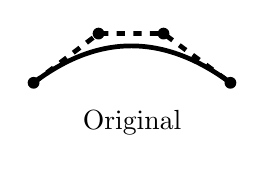
\begin{tikzpicture}[scale=2.5] 
\draw [line width=0.6mm, black ] (0, 0) .. controls (0.33,0.25) and (0.66,0.25)
   .. (1.0, 0.);
\fill (0,0) circle [radius=0.3mm];
\fill (0.33,0.25) circle [radius=0.3mm];
\fill (.66,.25) circle [radius=0.3mm];
\fill (1.,0) circle [radius=0.3mm];
\draw [line width=0.6mm, black,dashed ] (0,0) -- (0.33,0.25) -- (0.66,0.25) -- (1.,0);

\node at (0.5,-0.2) {Original};
\end{tikzpicture}
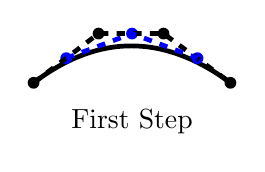
\begin{tikzpicture}[scale=2.5] 
\draw [line width=0.6mm, black ] (0, 0) .. controls (0.33,0.25) and (0.66,0.25)
   .. (1.0, 0.);
\fill (0,0) circle [radius=0.3mm];
\fill (0.33,0.25) circle [radius=0.3mm];
\fill (.66,.25) circle [radius=0.3mm];
\fill (1.,0) circle [radius=0.3mm];
\fill[fill=blue] (0.166,0.125) circle [radius=0.3mm];
\fill[fill=blue] (0.5,0.25) circle [radius=0.3mm];
\fill[fill=blue] (0.833,0.125) circle [radius=0.3mm];

\draw [line width=0.6mm, black,dashed ] (0,0) -- (0.33,0.25) -- (0.66,0.25) -- (1.,0);
\draw [line width=0.6mm, blue,dashed ] (0.166,0.125) -- (0.5,0.25) -- (0.833,0.125);

\node at (0.5,-0.2) {First Step};
\end{tikzpicture}
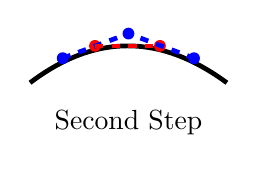
\begin{tikzpicture}[scale=2.5] 
\draw [line width=0.6mm, black ] (0, 0) .. controls (0.33,0.25) and (0.66,0.25)
   .. (1.0, 0.);
\fill[fill=blue] (0.166,0.125) circle [radius=0.3mm];
\fill[fill=blue] (0.5,0.25) circle [radius=0.3mm];
\fill[fill=blue] (0.833,0.125) circle [radius=0.3mm];
\fill[fill=red] (0.33,0.1875) circle [radius=0.3mm];
\fill[fill=red] (0.66,0.1875) circle [radius=0.3mm];
\draw [line width=0.6mm, blue,dashed ] (0.166,0.125) -- (0.5,0.25) -- (0.833,0.125);
\draw [line width=0.6mm, red,dashed ] (0.33,0.1875) -- (0.66,0.1875);

\node at (0.5,-0.2) {Second Step};
\end{tikzpicture}
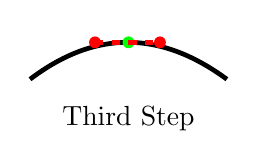
\begin{tikzpicture}[scale=2.5] 
\draw [line width=0.6mm, black ] (0, 0) .. controls (0.33,0.25) and (0.66,0.25)
   .. (1.0, 0.);
\fill[fill=red] (0.33,0.1875) circle [radius=0.3mm];
\fill[fill=red] (0.66,0.1875) circle [radius=0.3mm];
\fill[fill=green] (0.5,0.1875) circle [radius=0.3mm];

\draw [line width=0.6mm, red,dashed ] (0.33,0.1875) -- (0.66,0.1875);

\node at (0.5,-0.2) {Third Step};
\end{tikzpicture}
\end{figure}
\begin{figure}
\centering
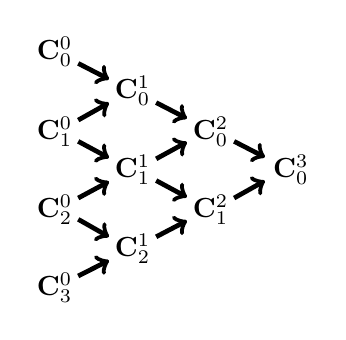
\begin{tikzpicture}[scale=3.0] 

\node at (0,1.0) {$\mathbf{C}^{0}_0$};
\node at (0,0.66) {$\mathbf{C}^{0}_1$};
\node at (0,0.33) {$\mathbf{C}^{0}_2$};
\node at (0,0) {$\mathbf{C}^{0}_3$};
\node at (0.33,0.833) {$\mathbf{C}^{1}_0$};
\node at (0.33,0.5) {$\mathbf{C}^{1}_1$};
\node at (0.33,0.166) {$\mathbf{C}^{1}_2$};
\node at (0.66,0.66) {$\mathbf{C}^{2}_0$};
\node at (0.66,0.33) {$\mathbf{C}^{2}_1$};
\node at (1.0,0.5) {$\mathbf{C}^{3}_0$};
\draw[line width=0.6mm,->] (0.1,0.95) -- (0.23,0.833+0.05);
\draw[line width=0.6mm,->] (0.1,0.95-0.33) -- (0.23,0.5+0.05);
\draw[line width=0.6mm,->] (0.1,0.95-0.66) -- (0.23,0.166+0.05);
\draw[line width=0.6mm,->] (0.1+0.33,0.95-0.166) -- (0.23+0.33,0.833+0.05-0.166);
\draw[line width=0.6mm,->] (0.1+0.33,0.95-0.33-0.166) -- (0.23+0.33,0.5+0.05-0.166);
\draw[line width=0.6mm,->] (0.1+0.66,0.95-0.33) -- (0.23+0.66,0.833+0.05-0.33);

\draw[line width=0.6mm,->] (0.1,0.05+0.66) -- (0.23,0.833-0.05);
\draw[line width=0.6mm,->] (0.1,0.05+0.33) -- (0.23,0.5-0.05);
\draw[line width=0.6mm,->] (0.1,0.05) -- (0.23,0.166-0.05);
\draw[line width=0.6mm,->] (0.1+0.33,0.05+0.33+0.166) -- (0.23+0.33,0.833-0.05-0.166);
\draw[line width=0.6mm,->] (0.1+0.33,0.05+0.166) -- (0.23+0.33,0.5-0.05-0.166);
\draw[line width=0.6mm,->] (0.1+0.66,0.05+0.33) -- (0.23+0.66,0.833-0.05-0.33);
\end{tikzpicture}
\end{figure}
The two new curves are comprised of points along the upper and lower of the diagram, $\mathbf{C}_0^{0},\mathbf{C}_0^{1},\mathbf{C}_0^{2},\mathbf{C}_0^{3}$, and
$\mathbf{C}_3^{0},\mathbf{C}_2^{1},\mathbf{C}_1^{2},\mathbf{C}_0^{3}$, where $\mathbf{C}_0^{3} = \mathbf{B}(u)$, it lies exactly on the original curve, at $u$.

\end{frame}
\begin{frame}{Subdivision - Curves}
Algorithmically, with the curves as $\mathbf{D}, \mathbf{E}$ we have that
{
  \footnotesize

\begin{algorithmic}
\State $\mathbf{D}_0 = \mathbf{C}^0_0$
\State $\mathbf{E}_P = \mathbf{C}^0_P$
\For{$i \in [0..P)$}
\For{$j \in [0..P-i)$}
\State $\mathbf{C}_j^{i+1} = (1-u)\mathbf{C}^i_j+u\mathbf{C}^i_{j+1}$
\EndFor
\State $\mathbf{D}_{i+1} = \mathbf{C}^{i+1}_{i+1}$
\State $\mathbf{E}_{P-i-1} = \mathbf{C}^{i+1}_{P-i-1}$
\EndFor
\end{algorithmic}
}
and we need to compute all intermediate control points to determine the subdivision. We also note that we could evaluate the curves at any $u$ using this method, and it is more stable, however the direct method is significantly faster. 
\end{frame}
\begin{frame}{Subdivision - Triangles}
Subdivision of triangles turns one triangle into three by splitting at some point $(u,v,w)$. Consider the third order triangle, with 10 points. The steps of the subdivision algorithm are shown on the right by subdividing each subtriangle, shown in red, blue, and green.
\begin{figure}
\centering
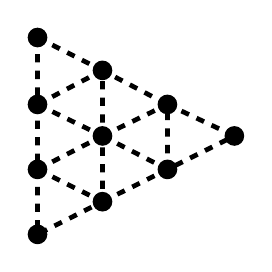
\begin{tikzpicture}[scale=2.5] 
\fill (0,1.0) circle [radius=0.5mm];
\fill (0,0.66) circle [radius=0.5mm];
\fill (0,0.33) circle [radius=0.5mm];
\fill (0,0) circle [radius=0.5mm];
\fill (0.33,0.833) circle [radius=0.5mm];
\fill (0.33,0.5) circle [radius=0.5mm];
\fill (0.33,0.166) circle [radius=0.5mm];
\fill (0.66,0.66) circle [radius=0.5mm];
\fill (0.66,0.33) circle [radius=0.5mm];
\fill (1.0,0.5) circle [radius=0.5mm];
\draw [line width=0.6mm, black,dashed ] (0,1.0) -- (0,0.66) -- (0,0.33) -- (0,0) -- (0.33,0.166) -- (0.33,0.5) 
-- (0.33,0.833) -- (0.66,0.66) -- (0.66,0.33) --(1.0,0.5) -- (0.66,0.66);
\draw [line width=0.6mm, black,dashed ] (0,1.0) -- (0.33,0.833);
\draw [line width=0.6mm, black,dashed ] (0,0.66) -- (0.33,0.5);
\draw [line width=0.6mm, black,dashed ] (0,0.33) -- (0.33,0.166);
\draw [line width=0.6mm, black,dashed ] (0.33,0.5)  -- (0.66,0.33);
\draw [line width=0.6mm, black,dashed ] (0.33,0.166)  -- (0.66,0.33);
\draw [line width=0.6mm, black,dashed ] (0.33,0.5)  -- (0.66,0.66);
\draw [line width=0.6mm, black,dashed ] (0,0.66) -- (0.33,0.833);
\draw [line width=0.6mm, black,dashed ] (0,0.33) -- (0.33,0.5);

\end{tikzpicture}
\begin{tikzpicture}[scale=2.5] 
\draw[line width=0.6mm,->] (0,0.5) -- (0.5,0.5);
\node at (0,0) {};
\end{tikzpicture}
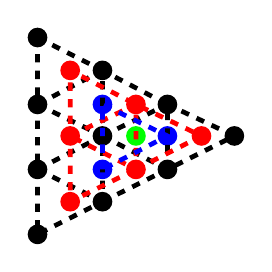
\begin{tikzpicture}[scale=2.5] 
\fill (0,1.0) circle [radius=0.5mm];
\fill (0,0.66) circle [radius=0.5mm];
\fill (0,0.33) circle [radius=0.5mm];
\fill (0,0) circle [radius=0.5mm];
\fill (0.33,0.833) circle [radius=0.5mm];
\fill (0.33,0.5) circle [radius=0.5mm];
\fill (0.33,0.166) circle [radius=0.5mm];
\fill (0.66,0.66) circle [radius=0.5mm];
\fill (0.66,0.33) circle [radius=0.5mm];
\fill (1.0,0.5) circle [radius=0.5mm];
\fill[fill=red] (0.166,0.166) circle [radius=0.5mm];
\fill[fill=red] (0.166,0.5) circle [radius=0.5mm];
\fill[fill=red] (0.166,0.833) circle [radius=0.5mm];

\fill[fill=red] (0.5,0.33) circle [radius=0.5mm];
\fill[fill=red] (0.5,0.66) circle [radius=0.5mm];
\fill[fill=red] (0.833,0.5) circle [radius=0.5mm];

\fill[fill=blue] (0.33,0.33) circle [radius=0.5mm];
\fill[fill=blue] (0.33,0.66) circle [radius=0.5mm];
\fill[fill=blue] (0.66,0.5) circle [radius=0.5mm];
\fill[fill=green] (0.5,0.5) circle [radius=0.5mm];

\draw [line width=0.6mm, black,dashed ] (0,1.0) -- (0,0.66) -- (0,0.33) -- (0,0) -- (0.33,0.166) -- (0.33,0.5) 
-- (0.33,0.833) -- (0.66,0.66) -- (0.66,0.33) --(1.0,0.5) -- (0.66,0.66);
\draw [line width=0.6mm, black,dashed ] (0,1.0) -- (0.33,0.833);
\draw [line width=0.6mm, black,dashed ] (0,0.66) -- (0.33,0.5);
\draw [line width=0.6mm, black,dashed ] (0,0.33) -- (0.33,0.166);
\draw [line width=0.6mm, black,dashed ] (0.33,0.5)  -- (0.66,0.33);
\draw [line width=0.6mm, black,dashed ] (0.33,0.166)  -- (0.66,0.33);
\draw [line width=0.6mm, black,dashed ] (0.33,0.5)  -- (0.66,0.66);
\draw [line width=0.6mm, black,dashed ] (0,0.66) -- (0.33,0.833);
\draw [line width=0.6mm, black,dashed ] (0,0.33) -- (0.33,0.5);


\draw [line width=0.6mm, red,dashed ] (0.5,0.33) -- (0.833,0.5) -- (0.5,0.66) -- (0.166,0.833) -- (0.166,0.5) -- (0.166,0.166) -- (0.5,0.33);
\draw [line width=0.6mm, red,dashed ] (0.166,0.5)  -- (0.5,0.66) -- (0.5,0.33) -- (0.166,0.5);
\draw [line width=0.6mm, blue,dashed ] (0.33,0.33)  -- (0.33,0.66)-- (0.66,0.5) -- (0.33,0.33);
\end{tikzpicture}
\end{figure}

\end{frame}
\begin{frame}{Subdivision - Triangles}
The three triangles, each with ten control points, are shown below.
\begin{figure}
\centering

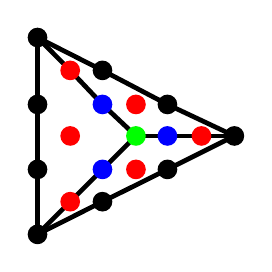
\begin{tikzpicture}[scale=2.5] 
\draw [line width=0.6mm] (0,1.0)  -- (0,0.66) -- (0,0.33) -- (0,0) -- (0.166,0.166) -- (0.33,0.33) -- 
(0.5,0.5) -- (0.33,0.66) -- (0.166,0.833) -- (0,1.0);
\draw [line width=0.6mm] (0,0) -- (0.33,0.166) -- (0.66,0.33) -- (1.0,0.5) -- (0.66,0.66) -- (0.33,0.833) -- (0,1.0);
\draw [line width=0.6mm] (1.0,0.5) -- (0.5,0.5);
\fill (0,1.0) circle [radius=0.5mm];
\fill (0,0.66) circle [radius=0.5mm];
\fill (0,0.33) circle [radius=0.5mm];
\fill (0,0) circle [radius=0.5mm];
\fill (0.33,0.833) circle [radius=0.5mm];
\fill (0.33,0.166) circle [radius=0.5mm];
\fill (0.66,0.66) circle [radius=0.5mm];
\fill (0.66,0.33) circle [radius=0.5mm];
\fill (1.0,0.5) circle [radius=0.5mm];
\fill[fill=red] (0.166,0.166) circle [radius=0.5mm];
\fill[fill=red] (0.166,0.5) circle [radius=0.5mm];
\fill[fill=red] (0.166,0.833) circle [radius=0.5mm];

\fill[fill=red] (0.5,0.33) circle [radius=0.5mm];
\fill[fill=red] (0.5,0.66) circle [radius=0.5mm];
\fill[fill=red] (0.833,0.5) circle [radius=0.5mm];

\fill[fill=blue] (0.33,0.33) circle [radius=0.5mm];
\fill[fill=blue] (0.33,0.66) circle [radius=0.5mm];
\fill[fill=blue] (0.66,0.5) circle [radius=0.5mm];
\fill[fill=green] (0.5,0.5) circle [radius=0.5mm];
\end{tikzpicture}
\end{figure}
The control points are 
\[\mathbf{C}^{n+1}_{i,j,k} = u\mathbf{C}^{n}_{i,j,k}+v\mathbf{C}^{n}_{i-1,j+1,k}+w\mathbf{C}^{n}_{i-1,j,k+1}\]
For each step of the algorithm. 
\end{frame}
\begin{frame}{Subdivision - Triangle}
In practice, subdivision at the triangle center $(1/3,1/3,1/3)$ is not ideal, since repeated subdivision does not converge (the longest edge of a triangle does not change). The classic option,
\begin{figure}
\centering

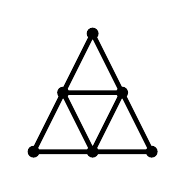
\begin{tikzpicture}[scale=1.5] 
\draw [line width=0.6mm] (0.5,1) -- (1,0) -- (0,0) -- (.5,1);
\draw [line width=0.6mm] (0.5,0) -- (0.25,0.5) -- (0.75,0.5) -- (0.5,0);

\fill (1.0,0) circle [radius=0.5mm];
\fill (0.5,0) circle [radius=0.5mm];
\fill (0,0) circle [radius=0.5mm];
\fill (0.25,.5) circle [radius=0.5mm];
\fill (0.75,.5) circle [radius=0.5mm];
\fill (0.5,1.0) circle [radius=0.5mm];

\end{tikzpicture}
\end{figure}
Can be obtained by four calls to the subdivision algorithm. First, denoting the three triangles in the split by
\begin{figure}
\centering

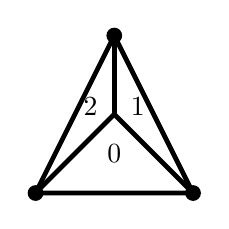
\begin{tikzpicture}[scale=2] 
\draw [line width=0.6mm] (0.5,1) -- (1,0) -- (0,0) -- (.5,1);
\draw [line width=0.6mm] (0.5,1.0) -- (0.5,0.5);
\draw [line width=0.6mm] (1.0,0) -- (0.5,0.5);
\draw [line width=0.6mm] (0,0) -- (0.5,0.5);

\fill (1.0,0) circle [radius=0.5mm];
\fill (0,0) circle [radius=0.5mm];
\fill (0.5,1.0) circle [radius=0.5mm];
\node at (0.5,0.25) {0};
\node at (0.65,0.55) {1};
\node at (0.35,0.55) {2};

\end{tikzpicture}
\end{figure}
\end{frame}
\begin{frame}{Subdivision - Triangles}
1. Split at (0.5,0.5,0).\\
2. Split 0 at (0,0.5,0.5).\\
3. Split 1 at (0,0.5,0.5).\\
4. Split 01 at (-1,1,1)
\begin{figure}
\centering

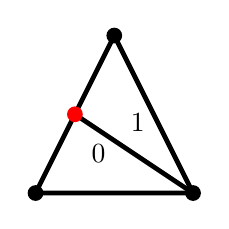
\begin{tikzpicture}[scale=2] 
\draw [line width=0.6mm] (0.5,1) -- (1,0) -- (0,0) -- (.5,1);
\draw [line width=0.6mm] (0.25,0.5) -- (1.0,0);

\fill (1.0,0) circle [radius=0.5mm];
\fill[fill=red] (0.25,0.5) circle [radius=0.5mm];
\fill (0,0) circle [radius=0.5mm];
\fill (0.5,1.0) circle [radius=0.5mm];
\node at (0.4,0.25) {0};
\node at (0.65,0.45) {1};
\end{tikzpicture}
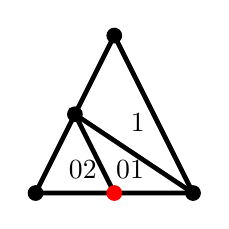
\begin{tikzpicture}[scale=2] 
\draw [line width=0.6mm] (0.5,1) -- (1,0) -- (0,0) -- (.5,1);
\draw [line width=0.6mm] (0.5,0) -- (0.25,0.5) -- (1.0,0);

\fill (1.0,0) circle [radius=0.5mm];
\fill (0.25,0.5) circle [radius=0.5mm];
\fill (0,0) circle [radius=0.5mm];
\fill (0.5,1.0) circle [radius=0.5mm];
\fill[fill=red] (0.5,0) circle [radius=0.5mm];

\node at (0.3,0.15) {02};
\node at (0.6,0.15) {01};

\node at (0.65,0.45) {1};
\end{tikzpicture}
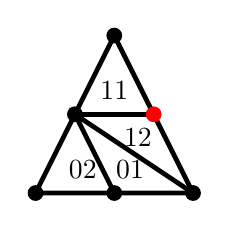
\begin{tikzpicture}[scale=2] 
\draw [line width=0.6mm] (0.5,1) -- (1,0) -- (0,0) -- (.5,1);
\draw [line width=0.6mm] (0.5,0) -- (0.25,0.5) -- (1.0,0);
\draw [line width=0.6mm] (0.25,0.5) -- (0.75,0.5);

\fill (1.0,0) circle [radius=0.5mm];
\fill (0.25,0.5) circle [radius=0.5mm];
\fill (0,0) circle [radius=0.5mm];
\fill (0.5,1.0) circle [radius=0.5mm];
\fill (0.5,0) circle [radius=0.5mm];
\fill[fill=red] (0.75,0.5) circle [radius=0.5mm];

\node at (0.3,0.15) {02};
\node at (0.6,0.15) {01};

\node at (0.65,0.35) {12};
\node at (0.5,0.65) {11};

\end{tikzpicture}
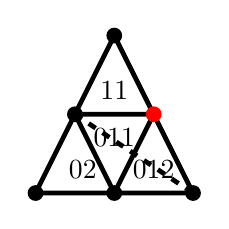
\begin{tikzpicture}[scale=2] 
\draw [line width=0.6mm] (0.5,1) -- (1,0) -- (0,0) -- (.5,1);
\draw [line width=0.6mm,dashed] (0.25,0.5) -- (1.0,0);
\draw [line width=0.6mm] (0.5,0) -- (0.25,0.5) -- (0.75,0.5);
\draw [line width=0.6mm] (0.5,0) -- (0.75,0.5);

\fill (1.0,0) circle [radius=0.5mm];
\fill (0.25,0.5) circle [radius=0.5mm];
\fill (0,0) circle [radius=0.5mm];
\fill (0.5,1.0) circle [radius=0.5mm];
\fill (0.5,0) circle [radius=0.5mm];
\fill[fill=red] (0.75,0.5) circle [radius=0.5mm];

\node at (0.3,0.15) {02};
\node at (0.75,0.15) {012};

\node at (0.5,0.35) {011};
\node at (0.5,0.65) {11};

\end{tikzpicture}
\end{figure}
The issue with this split is that it requires a non convex call (-1,1,1), but in practice, this has been shown to work.
\end{frame}
\begin{frame}{Subdivision - Matrices}
Subdivision can also be computed with matrices, as is done by Remacle and others. Consider the subdivision of a curve, creating a new curve from $\xi = a$ to $\xi = b$, $0 < a < b < 1$. Define $\xi_s = a+(b-a)\xi$, we can write the control points of the new curve, $\mathbf{C}_s$, in terms of the old curve as
\[
\mathbf{B}(\xi_s)\mathbf{C} = \mathbf{B}(\xi)\mathbf{C}_s
\]
The control points are then 
\[ 
\mathbf{C}_s = \mathbf{B}^{-1}\mathbf{B}_s \mathbf{C}
\]
With $\mathbf{B}_s = \mathbf{B}(\xi_s)$ and $\mathbf{B}^{-1}\mathbf{B}_s$ is the subdivision matrix for that particular subdivision. To subdivide a tetrahedron into 8 tetrahedra, for validity checking, the ranges are given in \texttt{crvBezierPoints.cc}.
\end{frame}
\section{Derivatives}
\begin{frame}{Derivatives of a Curve}
The derivatives of a B{\'e}zier curve as also a B{\'e}zier curve, writing the formula as a function of just $u$,
\[ \mathbf{B}(u) = \displaystyle \sum_{i=0}^{P} {P \choose i}u^i(1-u)^{P-i}\mathbf{C}_{i}   \]
The derivative is an order $P-1$ B{\'e}zier, of the form 
\[
\frac{\mathrm{d} \mathbf{B}(u)}{\mathrm{d} u} = P \displaystyle\sum_{i=0}^{P-1}  {P-1 \choose i}u^i(1-u)^{P-1-i}(\mathbf{C}_{i+1}-\mathbf{C}_i)
\]
Implementation wise, it is easier to evaluate it based on just the control points themselves, as
{
  \footnotesize
\[
\frac{\mathrm{d} \mathbf{B}(u)}{\mathrm{d} u} = -P(1-u)^{P-1}\mathbf{C}_0+\displaystyle \sum_{i=1}^{P-1} {P \choose i}(i-Pu)u^{i-1}(1-u)^{P-i-1}\mathbf{C}_i + Pu^{P-1}\mathbf{C}_P
\]
}
The derivatives of a triangle and tet are written out similarly, as sums of derivatives of the weights of each control point.
\end{frame}
\section{Blended Shapes}
\begin{frame}{Blended Triangles}
The blended triangle is a transfinite interpolation of triangle edges, of the form
\[\mathbf{x}(\xi) = \sum_{i=0}^{3}||\xi_{e_i}||w_{e_i}(\xi_{e_i})\mathbf{x}(\xi_{e_i}) - \sum_{i=0}^{3}\xi_i\mathbf{x}_{v_i}\]
We can use this on all triangles not on a boundary, triangular blending of shape functions can be used. This occurs for all 2D triangles and 3D interior triangles with an edge or more on the boundary.
\end{frame}
\begin{frame}{Blended Triangles}
For a given entity on the mesh, we can write the shape as
\[ \mathbf{x}(\xi) = \sum_{i=0}^N w_i(\xi) \mathbf{x}_i \]
for an entity with $N$ total nodes, where $\xi = (u,v,w)$. For example, for B{\'e}zier shapes, $w_i(\xi) = B_{\mathbf{i}}(\xi)$ To implement the blending in our framework, we have 
\[\mathbf{x}_{face}(\xi) = \sum_{i=0}^{3}||\xi_{e_i}||\sum_{j=0}^{N_{edge}}w_{e_i,j}(\xi_{e_i})\cdot\mathbf{x}_{e_i,j}- \sum_{i=0}^{3}\xi_i\mathbf{x}_{v_i}\]
\end{frame}
\begin{frame}{Blended Triangles}
The edge parameters are
\begin{eqnarray*} 
\xi_{e_0} & = & \frac{\xi_1}{\xi_0+\xi_1},\quad ||\xi_{e_0}|| = \xi_0+\xi_1 \\
\xi_{e_1} & = & \frac{\xi_2}{\xi_1+\xi_2},\quad ||\xi_{e_1}|| = \xi_1+\xi_2 \\
\xi_{e_2} & = & \frac{\xi_0}{\xi_2+\xi_0},\quad ||\xi_{e_2}|| = \xi_2+\xi_0 
\end{eqnarray*}
Based on the canonical ordering of edges and faces. When any of $||\xi_{e_i}|| = 0$, $\frac{\xi_1}{\xi_0+\xi_1} = \frac{1}{2}$, the midpoint of the edge. This is irrelevant for the actual shape, but important in computing derivatives.
\end{frame}
\begin{frame}{Blended Triangles}

The goal is then to find face weights such that \[\mathbf{x}_{face}(\xi) = \sum_{i=0}^{N_{face}} w_i(\xi) \cdot \mathbf{x}_i = \sum_{i=0}^{3}||\xi_{e_i}||\sum_{j=0}^{N_{edge}}w_{e_i,j}(\xi_{e_i})\cdot\mathbf{x}_{e_i,j}- \sum_{i=0}^{3}\xi_i\mathbf{x}_{v_i} \] 
This is a bookkeeping exercise, since every $x_{e_i,j}$ corresponds to a point on the face, in $x_i$. 
\end{frame}
\begin{frame}{Blended Triangles}
\begin{figure}
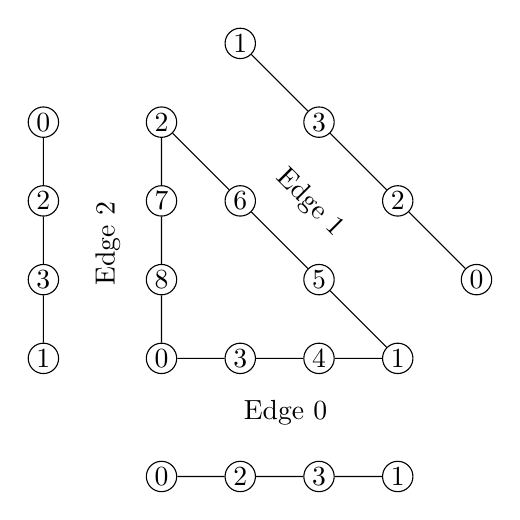
\begin{tikzpicture}[scale=1]
\tikzstyle{every node}=[circle, draw, fill=white,
                        inner sep=1pt, minimum width=4pt]
\path (0,0) node (p0) {$0$}
(1,0) node [label={[label distance=0.1cm]-60:Edge 0}] (p1) {$3$}
(2,0) node (p2) {$4$}
(3,0) node (p3) {$1$}
(2,1) node (p4) {$5$}
(1,2) node [label={[label distance=0.1cm,rotate=-45]10:Edge 1}] (p5) {$6$}
(0,3) node (p6) {$2$}
(0,2) node [label={[label distance=0.2cm,rotate=90]-200:Edge 2}] (p7) {$7$}
(0,1) node (p8) {$8$}
(0,-1.5) node (p10) {$0$}
(1,-1.5) node (p11) {$2$}
(2,-1.5) node (p12) {$3$}
(3,-1.5) node (p13) {$1$}
(-1.5,0) node (p14) {$1$}
(-1.5,1) node (p15) {$3$}
(-1.5,2) node (p16) {$2$}
(-1.5,3) node (p17) {$0$}
(1,4) node (p18) {$1$}
(2,3) node (p19) {$3$}
(3,2) node (p20) {$2$}
(4,1) node (p21) {$0$};
\draw (p0) -- (p1)
(p1) -- (p2)
(p2) -- (p3)
(p3) -- (p4)
(p4) -- (p5)
(p5) -- (p6)
(p6) -- (p7)
(p7) -- (p8)
(p8) -- (p0)
(p10) -- (p11)
(p11) -- (p12)
(p12) -- (p13)
(p14) -- (p15)
(p15) -- (p16)
(p16) -- (p17)
(p18) -- (p19)
(p19) -- (p20)
(p20) -- (p21);
\end{tikzpicture}
\end{figure}
\end{frame}
\begin{frame}{Blended Triangles}
The face has 9 nodes associated with it, ordered as shown. The weights are then 
\begin{eqnarray*}
w_0 & = & ||\xi_{e_0}||w_{e_0,0}(\xi_{e_0}) + ||\xi_{e_2}||w_{e_2,1}(\xi_{e_2}) - \xi_0 \\
w_1 & = & ||\xi_{e_0}||w_{e_0,1}(\xi_{e_0}) + ||\xi_{e_1}||w_{e_1,0}(\xi_{e_1}) - \xi_1 \\
w_2 & = & ||\xi_{e_2}||w_{e_2,0}(\xi_{e_2}) + ||\xi_{e_1}||w_{e_1,1}(\xi_{e_1}) - \xi_2 \\
w_3 & = & ||\xi_{e_0}||w_{e_0,2}(\xi_{e_0}) \\
w_4 & = & ||\xi_{e_0}||w_{e_0,3}(\xi_{e_0}) \\
w_5 & = & ||\xi_{e_1}||w_{e_1,2}(\xi_{e_1}) \\
w_6 & = & ||\xi_{e_1}||w_{e_1,3}(\xi_{e_1}) \\
w_7 & = & ||\xi_{e_2}||w_{e_2,2}(\xi_{e_2}) \\
w_8 & = & ||\xi_{e_2}||w_{e_2,3}(\xi_{e_2})
\end{eqnarray*}
Where, for example, $w_{e_0,0}(\xi_{e_0}) = B_{21}(\xi_{e_0})$.
\end{frame}
\begin{frame}{Blended Triangles}
The local gradients are then
\begin{eqnarray*}\frac{\partial \mathbf{x}(\xi)}{\partial \xi_k}& = & \sum_{i=0}^N \frac{\partial w_i(\xi)}{\partial \xi_k} \cdot \mathbf{x}_i \\
\frac{\partial \mathbf{x}(\xi)}{\partial \xi_k}& = & \frac{\partial}{\partial \xi_k}\left[\sum_{i=0}^{3}||\xi_{e_i}||\sum_{j=0}^{N_{edge}}w_{e_i,j}(\xi_{e_i})\cdot\mathbf{x}_{e_i,j}- \sum_{i=0}^{3}\xi_i\mathbf{x}_{v_i}\right] \\ & & 
\sum_{i=0}^{3}\frac{\partial}{\partial \xi_k}\left[||\xi_{e_i}||\sum_{j=0}^{N_{edge}}w_{e_i,j}(\xi_{e_i})\right]\cdot\mathbf{x}_{e_i,j}- \sum_{i=0}^{3} \frac{\partial \xi_i}{\partial \xi_k}\mathbf{x}_{v_i}\end{eqnarray*}
\end{frame}
\begin{frame}{Blended Triangles}
{
  \footnotesize
For the vertex terms, we have
\[ \frac{\partial \xi_i}{\partial \xi_k} = \left[ \begin{array}{ccc} 1 & 0 & 0 \\ 0 & 1 & 0 \\ -1 & -1 & 0 \end{array}\right]\]
and for the edge terms, the chain rule leads to


\begin{eqnarray*}
\frac{\partial}{\partial \xi_k}\left[||\xi_{e_i}||\sum_{j=0}^{N_{edge}}w_{e_i,j}(\xi_{e_i})\right] & = & \frac{\partial ||\xi_{e_i}||}{\partial \xi_k}\sum_{j=0}^{N_{edge}}w_{e_i,j}(\xi_{e_i}) \\ & + & ||\xi_{e_i}||\sum_{j=0}^{N_{edge}}\frac{\partial w_{e_i,j}(\xi_{e_i})}{\partial \xi_k}
\end{eqnarray*}

where the first term is straight forward, and the second term, 
\begin{eqnarray*}
||\xi_{e_i}||\frac{\partial w_{e_i,j}(\xi_{e_i})}{\partial \xi_k} & = &
||\xi_{e_i}||\frac{\partial w_{e_i,j}(\xi_{e_i})}{\partial \xi_{e_i}}\frac{\partial \xi_{e_i}}{\partial \xi_k} 
\\ & = & 
||\xi_{e_i}||\frac{\partial w_{e_i,j}(\xi_{e_i})}{\xi_{e_i}}\left[\frac{\partial \xi_{e_i}'}{\partial \xi_k}||\xi_{e_i}||-\xi_{e_i}'\frac{\partial ||\xi_{e_i}||}{\partial \xi_k} \right]
\end{eqnarray*}
}
\end{frame}
\begin{frame}{Blended Triangles}{Continuity}
The linear blending, with $k = 1$ is not continuous across edges. To increase the order of continuity, Dey suggests a general form
\[\mathbf{x}(\xi) = \sum_{i=0}^{3}||\xi_{e_i}||^kw_{e_i}(\xi_{e_i})\mathbf{x}(\xi_{e_i}) - \sum_{i=0}^{3}\xi_i^k\mathbf{x}_{v_i}\]
However, this is only useful up to $k = 2$, where the blending no longer preserves a linear element.
\end{frame}
\begin{frame}{Blended Triangles}
Consider a linear triangle, with vertices $\mathbf{v}_0,\mathbf{v}_1,\mathbf{v}_2$ and barycentric coordinates $u,v,w$. We can write the blending as
\begin{eqnarray*}
\mathbf{x} & = &(u+v)^k\left(\left(1-\frac{v}{u+v}\right)\mathbf{v}_0 + \frac{v}{u+v}\mathbf{v}_1\right) + \\
&&(v+w)^k\left(\left(1-\frac{w}{v+w}\right)\mathbf{v}_1 + \frac{w}{v+w}\mathbf{v}_2\right) + \\
&&(w+u)^k\left(\left(1-\frac{u}{w+u}\right)\mathbf{v}_2 + \frac{u}{w+u}\mathbf{v}_0\right) + \\
&&-u^k\mathbf{v}_0-v^k\mathbf{v}_1-w^k\mathbf{v}_2
\end{eqnarray*}
\end{frame}
\begin{frame}{Blended Triangles}
We can rewrite this as
\begin{eqnarray*}
\mathbf{x} & = &(u+v)^{k-1}\left(u\mathbf{v}_0 + v\mathbf{v}_1\right) + \\
&&(v+w)^{k-1}\left(v\mathbf{v}_1 + w\mathbf{v}_2\right) + \\
&&(w+u)^{k-1}\left(w\mathbf{v}_2 + u\mathbf{v}_0\right) + \\
&&-u^k\mathbf{v}_0-v^k\mathbf{v}_1-w^k\mathbf{v}_2
\end{eqnarray*}
for $k = 1$, we reduce to the exact linear mapping.
\[
\mathbf{x} = u\mathbf{v}_0+v\mathbf{v}_1+w\mathbf{v}_2
\]

For $k = 2$, we again reduce to the exact linear mapping.
\[
\mathbf{x} = (u\mathbf{v}_0+v\mathbf{v}_1+w\mathbf{v}_2)(u+v+w) = u\mathbf{v}_0+v\mathbf{v}_1+w\mathbf{v}_2
\]
\end{frame}
\begin{frame}{Blended Triangles}
For $k = 3$, we get
\[
\mathbf{x} = (u^3 + 2u^2v + 2u^2w + uv^2 + uw^2)\mathbf{v}_0
\]
Which is a valid mapping, but does not preserve the linear behavior we would hope for.
Of interest is if there exists a function $g(x)$ such that the linear behavior is preserved for all $k$.
\begin{eqnarray*}
\mathbf{x} & = &g(u+v)^k\left(\left(1-\frac{v}{u+v}\right)\mathbf{v}_0 + \frac{v}{u+v}\mathbf{v}_1\right) + \\
&&g(v+w)^k\left(\left(1-\frac{w}{v+w}\right)\mathbf{v}_1 + \frac{w}{v+w}\mathbf{v}_2\right) + \\
&&g(w+u)^k\left(\left(1-\frac{u}{w+u}\right)\mathbf{v}_2 + \frac{u}{w+u}\mathbf{v}_0\right) + \\
&&-u^k\mathbf{v}_0-v^k\mathbf{v}_1-w^k\mathbf{v}_2
\end{eqnarray*}
\end{frame}
\begin{frame}{Blended Triangles}
The goal would be to find a $g(x)$ such that 
\[\mathbf{x} = (u\mathbf{v}_0+v\mathbf{v}_1+w\mathbf{v}_2)(u+v+w)^{k-1} \]
which reduces to the linear mapping. If we consider the coefficient of the first vertex $\mathbf{v}_0$, we get
\[\left(g(u+v)^k\left(1-\frac{v}{u+v}\right)+g(w+u)^k\frac{u}{w+u}-u^k\right)\]
Observing that $ (u+v+w)^{k-1} = (vw^{k-2}+\ldots+v^{k-2}w) + \ldots$, we note that there is no way for the coefficient of $\mathbf{v}_0$ to contain a $vw$ term, and therefore this formulation makes it impossible to preserve the linear triangle for all $k$, specifically $k > 2$.
\end{frame}
\begin{frame}{Blended Tetrahedra}
For blended tetrahedra, we have
\[\mathbf{x}(\xi) = \sum_{i=0}^{4}||\xi_{f_i}||w_{f_i}(\xi_{f_i})\mathbf{x}(\xi_{f_i}) - \sum_{i=0}^{6}||\xi_{e_i}||w_{e_i}(\xi_{e_i})\mathbf{x}(\xi_{e_i}) + \sum_{i=0}^{4}\xi_i\mathbf{x}_{v_i}\]
The math is identical to triangles, though more consideration to ordering is needed, specifically the face contributions from their edges.
Similar to triangles, when any of $||\xi_{e_i}|| = 0$, $\frac{\xi_1}{\xi_0+\xi_1} = \frac{1}{2}$ for edges and now when $||\xi_{e_f}|| = 0$, $\frac{\xi_0}{\xi_0+\xi_1+\xi_2} = \frac{1}{3}$, again, only relevant when taking derivatives.
\end{frame}
\section{Interpolating B{\'e}zier Shapes}
\begin{frame}{Interpolating B{\'e}zier Triangles}
To fit a B{\'e}zier triangle to a known geometry, interpolating points, $\mathbf{P}_{ijk} =\mathbf{P}_{\mathbf{i}} = \mathbf{B}(\xi) =\mathbf{B}(u,v,w)$, are first needed at $\xi_0,\ldots, \xi_{N}$, for $N$ total interpolation points before the control points can be calculated. To simplify notation, $\mathbf{i} = ijk$. We can write the triangle as

\[
\mathbf{B}(\xi_j) = \displaystyle \sum_{|{\mathbf{i}| = P}} B_\mathbf{i}(\xi_j)\mathbf{C}_{\mathbf{i}} = \mathbf{P}_{\mathbf{i}}
\]
at each interpolating point, resulting in a linear system of equations for $\mathbf{C}_i$,
\[
\mathbf{P} = \mathbf{B}(\xi_j)\mathbf{C}
\]
The control points are then $\mathbf{C} = \mathbf{B}^{-1}(\xi_j)\mathbf{P}$. 
\end{frame}
\begin{frame}
For each set of $\xi_j$, we can precompute and store $\mathbf{B}^{-1}(\xi_j)$. Due to the structure of $\mathbf{B}$ and since edges of B{\'e}zier triangles are B{\'e}zier curves, we only need to store the rows of $\mathbf{B}^{-1}(\xi_j)$ for the internal points of the triangle, a $\frac{(P-1)(P-2)}{2} \times \frac{(P+1)(P+2)}{2}$ matrix. For edges, a $(P-1) \times (P+1)$ matrix is stored. \spa
To convert interpolation points to control points, the internal triangle control points are computed and then the edge control points. This avoids storing both sets of points. \spa
Several choices of $\xi_j$ exist. Using equally spaced $\xi_j$'s works fairly well, but closer to optimal points are in a paper by Chen and Babuska, 1995.
\end{frame}
\begin{frame}{Computing Internal Control Points of Full B{\'e}zier Shapes}
For a B{\'e}zier triangle or tetrahedra that has a curved boundary (edges or faces), the internal control points should be placed at a suitable location in parametric space. Without a parametrized geometry to interpolate, shape blending is used to determine the internal interpolation points. \spa
% \begin{figure}
% \centering
% \begin{tikzpicture}[scale=3.0] 
% \draw [line width=0.6mm, black ] (0, 0) .. controls (0.5,-0.25) and (1.0, -0.25)
%    .. (1.5, 0.) .. controls (1.25,0.6) and (1.0,0.8) 
%    .. (0.75,1.) .. controls (0.5,0.8) and (0.25,0.6) 
%    .. (0,0); 

% \path (-0.1,-0.1) node {$\mathbf{C}_{300}$}
% (0.375,-0.35) node {$\mathbf{C}_{210}$}
% (1.175,-0.37) node {$\mathbf{C}_{120}$}
% (1.6,-0.13) node {$\mathbf{C}_{030}$}
% (1.45,0.55) node {$\mathbf{C}_{021}$}
% (1.22,0.85) node {$\mathbf{C}_{012}$}
% (0.75,1.15) node {$\mathbf{C}_{003}$}
% (0.1,0.55) node {$\mathbf{C}_{201}$}
% (0.3,0.85) node {$\mathbf{C}_{102}$}
% (0.75,0.5) node {$\mathbf{C}_{111}$};
% \fill (0,0) circle [radius=0.5mm];
% \fill (0.5,-0.25) circle [radius=0.5mm];
% \fill (1.0,-.25) circle [radius=0.5mm];
% \fill (1.5,0) circle [radius=0.5mm];
% \fill (1.25,0.6) circle [radius=0.5mm];
% \fill (1.0,0.8) circle [radius=0.5mm];
% \fill (0.5,0.8) circle [radius=0.5mm];
% \fill (0.25,0.6) circle [radius=0.5mm];
% \fill (0.75,0.3) circle [radius=0.5mm];
% \fill (0.75,1.) circle [radius=0.5mm];

% \end{tikzpicture}
% \end{figure}
% \end{frame}
% \begin{frame}{Computing Internal Control Points}
We choose a set of local parametric locations, $\xi_j$, one for each internal point. We can determine this interpolation point using our blended shapes. 
\end{frame}
\begin{frame}{Computing Internal Control Points}
Write the blended shape as 
\[\mathbf{P}(\xi) = \displaystyle \sum_{\mathbf{i} \in shape\;boundaries}Bl_{\mathbf{i}}(\xi)\mathbf{C}_\mathbf{i}\] 
where the control points on the shape boundaries have been determined from interpolating locations along the bounding entities. The equation to solve is then
\[ \mathbf{P}(\xi) = \displaystyle \sum_{\mathbf{i} \in shape\;boundaries}Bl_{\mathbf{i}}(\xi)\mathbf{C}_\mathbf{i} = \displaystyle \sum_{|{\mathbf{i}| = P}} B_\mathbf{i}(\xi)\mathbf{C}_{\mathbf{i}} \]
This is an equation for the internal points $\mathbf{C}_{ijk(l)}, i > 0, j>0, k>0, (l > 0), i+j+k(+l) = P$.
\end{frame}
\begin{frame}{Computing Internal Control Points}
 \[\displaystyle \sum_{\mathbf{i} \in shape\;boundaries}(Bl_{\mathbf{i}}(\xi)-B_\mathbf{i}(\xi))\mathbf{C}_\mathbf{i} = \displaystyle \sum_{\mathbf{i} \in internal\;points} B_\mathbf{i}(\xi)\mathbf{C}_{\mathbf{i}} \]
 Which is a system of equations the size of the number of internal points. We can now solve for those locations. In matrix form, setting $Bl_\mathbf{i} = 0$ for the internal control points, we can write the equation for all the control points as
\[\mathbf{C} = \mathbf{B}^{-1}\mathbf{Bl}, \qquad \mathbf{B}^{-1}\mathbf{Bl} = \left[\begin{array}{cc}\mathbf{I} & \mathbf{0} \\ \mathbf{A}  &\mathbf{0} \end{array}\right] \]
and $\mathbf{A}$ is of size (number of internal points)$\times$(number of boundary points). We can precompute $\mathbf{A}$ for each set of $(\xi)$, and store it, applying it to the control points of each internal entity. This determines the control points for a B{\'ezier} shape on the interior. (This is similar to P.L. George's approach for serendipity shapes).

\end{frame}
\section{Jacobian Determinants}
\begin{frame}{Jacobian Determinants - Triangle}
The Jacobian Determinant is itself a B{\'e}zier shape. Consider a triangle in $x-y$, we have
\[
\mathbf{J} = \frac{\partial \mathbf{B}(u,v)}{\partial \mathbf{x}} = 
\left[\begin{array}{cc} \frac{\partial B_x}{\partial x} & \frac{\partial B_x}{\partial y}  \\
\frac{\partial B_y}{\partial x} & \frac{\partial B_y}{\partial y} \end{array} \right]
\]
As the derivative is one order lower, we get
\[
\mathbf{J} = \frac{\partial \mathbf{B}(u,v)}{\partial \mathbf{x}} = 
\left[\begin{array}{cc} \mathcal{O}(P-1) & \mathcal{O}(P-1) \\ \mathcal{O}(P-1) & \mathcal{O}(P-1) \end{array} \right]
\]
And thus the determinant for a tet, denoted $\det(\mathbf{J}) = \mathcal{J}(u,v)$, is $\mathcal{J} = \mathcal{O}(2(P-1))$. If the $\mathcal{J} > 0$ everywhere, the element is valid, otherwise it is invalid.
\end{frame}
\begin{frame}{Jacobian Determinants - Triangle}
To evaluate $\mathcal{J}(u,v)$, one option is to compute it directly. Writing the triangle as
 \[ \mathbf{B}(u,v) = \displaystyle\sum_{i+j+k=P} \frac{P!}{i!j!k!}u^iv^j(1-u-v)^k\mathbf{C}_{ijk} \]
 and the derivative vector of its coefficients at each control point, with $\mathbf{u} = (u,v)$
  \[ \frac{\partial B(\mathbf{u})_{ijk}}{\partial \mathbf{u}} =\frac{P!}{i!j!k!} \frac{\partial}{\partial \mathbf{u}}\left( u^iv^j(1-u-v)^k\right) \]
The Jacobian matrix is
\[\mathbf{J}(\mathbf{u}) = \displaystyle\sum_{i+j+k=P}\mathbf{C}_{ijk} \otimes \frac{\partial B(\mathbf{u})_{ijk}}{\partial \mathbf{u}} \]
and the determinant is straightforward.
\end{frame}
\begin{frame}{Jacobian Determinants - Triangle}
The other way to compute it is by first calculating the B{\'e}zier form of $\mathcal{J}$, and then evaluating it. 
{
  \footnotesize

\[ \mathcal{J}(u,v) = \displaystyle\sum_{I+J+K+L=2(P-1)}  {2(P-1) \choose I,J,K}u^Iv^J(1-u-v)^KN_{IJK}  \]
}where the control points, $N_{IJK}$, (scalars) are sums of determinants of the control points
{
  \scriptsize
\begin{eqnarray*}
N_{IJK} = P^2 \displaystyle\sum_{|i|=I,|j|=J,|k|=K} \frac{{P-1 \choose i_1,j_1}{P-1 \choose i_2,j_2}}{ {2(P-1) \choose I,J,K}} \\  \times|\mathbf{C}_{i_1+1,j_1,k_1}-\mathbf{C}_{i_1,j_1+1,k_1},\mathbf{C}_{i_2+1,j_2,k_2}-\mathbf{C}_{i_2,j_2,k_2+1}|
\end{eqnarray*}
\[|i| = i_1+i_2, |j| = j_1+j_2, |k| = k_1+k_2, \qquad i_1+j_1+k_1 = i_2+j_2+k_2 = P-1\]
}
\end{frame}
\begin{frame}{Jacobian Determinants - Triangle}
Since $\mathcal{J}$ is order $2(P-1)$, the number of control points $N_{IJK}$ is much higher than the number of control points of the original shape. In this table, "Terms" is the number of determinants calculated to compute the control points.

\begin{tabular}{|cc|ccc|}
\hline \multicolumn{2}{|c|}{B{\'e}zier Triangle} & \multicolumn{3}{|c|}{Jacobian Determinant} \\ \hline
Order & Num Ctrl Pts & Order & Num Ctrl Pts & Terms \\ 
\hline 1 & 3 & 0 & 1 & 1 \\
2 & 6 & 2 & 6 & 9 \\
3 & 10 & 4 & 15 & 36 \\
4 & 15 & 6 & 28 & 100 \\
5 & 21 & 8 & 45 & 225 \\
6 & 28 & 10 & 66 & 441 \\
7 & 36 & 12 & 91 & 784 \\ \hline
\end{tabular}
\end{frame}

\begin{frame}{Jacobian Determinants - Triangle}
For a second order triangle, the Jacobian determinant is also second order, with control points
\begin{eqnarray*}
N_{200}&=&4\left|\mathbf{C}_{110}-\mathbf{C}_{200},\mathbf{C}_{101}-\mathbf{C}_{200}\right|
\\N_{020}&=&4\left|\mathbf{C}_{020}-\mathbf{C}_{110},\mathbf{C}_{011}-\mathbf{C}_{110}\right|
\\N_{002}&=&4\left|\mathbf{C}_{011}-\mathbf{C}_{101},\mathbf{C}_{002}-\mathbf{C}_{101}\right|
\\N_{110}&=&2\left|\mathbf{C}_{110}-\mathbf{C}_{200},\mathbf{C}_{011}-\mathbf{C}_{110}\right|+\\&&2\left|\mathbf{C}_{020}-\mathbf{C}_{110},\mathbf{C}_{101}-\mathbf{C}_{200}\right|
\\N_{011}&=&2\left|\mathbf{C}_{011}-\mathbf{C}_{101},\mathbf{C}_{011}-\mathbf{C}_{110}\right|+\\&&2\left|\mathbf{C}_{020}-\mathbf{C}_{110},\mathbf{C}_{002}-\mathbf{C}_{101}\right|
\\N_{101}&=&2\left|\mathbf{C}_{011}-\mathbf{C}_{101},\mathbf{C}_{101}-\mathbf{C}_{200}\right|+\\&&2\left|\mathbf{C}_{110}-\mathbf{C}_{200},\mathbf{C}_{002}-\mathbf{C}_{101}\right|
\end{eqnarray*}
\end{frame}
% \begin{frame}{Jacobian Determinants - Triangle}
% \begin{figure}
% \centering
% \begin{tikzpicture}
% [x={(-0.866cm,-0.5cm)}, y={(0.866cm,-0.5cm)}, z={(0cm,1cm)}, scale=3.0]

% \draw [line width=0.3mm,->,red](0,0,0) -- (1.3,0,0);
% \node at (1.4,0,0) {$u$};
% \draw [line width=0.3mm,->,red](0,0,0) -- (0,1.3,0);
% \node at (0,1.4,0) {$v$};
% \draw [line width=0.3mm,<->,red](0,0,-0.5) -- (0,0,0.5);
% \node at (0,0,0.6) {$\mathcal{J}$};
% \draw [line width=0.6mm] (0,1,0.2) -- (1,0,0.2) -- (0,0,0.2) -- (0,1,0.2);
% \draw [line width=0.6mm] (0.5,0,0.1) -- (0.5,0.5,-.2) -- (0,0.5,0.1) -- (0.5,0,0.1);

% \fill (1.0,0,0.2) circle [radius=0.5mm];
% \fill (0.5,0,0.1) circle [radius=0.5mm];
% \fill (0,0,0.2) circle [radius=0.5mm];
% \fill (0,.5,0.1) circle [radius=0.5mm];
% \fill (0.5,.5,-.2) circle [radius=0.5mm];
% \fill (0,1.0,0.2) circle [radius=0.5mm];



% \end{tikzpicture}
% \end{figure}
% \end{frame}

\begin{frame}{Jacobian Determinants - Triangle}
For a third order triangle, the Jacobian determinant is fourth order, with 15 control points, the first 12, corresponding to the vertices and edges of the determinant are
{
  \scriptsize

\begin{eqnarray*}
N_{400}&=&9\left|\mathbf{C}_{210}-\mathbf{C}_{300},\mathbf{C}_{201}-\mathbf{C}_{300}\right|
\\N_{040}&=&9\left|\mathbf{C}_{030}-\mathbf{C}_{120},\mathbf{C}_{021}-\mathbf{C}_{120}\right|
\\N_{004}&=&9\left|\mathbf{C}_{012}-\mathbf{C}_{102},\mathbf{C}_{003}-\mathbf{C}_{102}\right|
\\N_{310}&=&4\left|\mathbf{C}_{210}-\mathbf{C}_{300},\mathbf{C}_{111}-\mathbf{C}_{210}\right|+4\left|\mathbf{C}_{120}-\mathbf{C}_{210},\mathbf{C}_{201}-\mathbf{C}_{300}\right|
\\N_{220}&=&\left|\mathbf{C}_{210}-\mathbf{C}_{300},\mathbf{C}_{021}-\mathbf{C}_{120}\right|+6\left|\mathbf{C}_{120}-\mathbf{C}_{210},\mathbf{C}_{111}-\mathbf{C}_{210}\right|+\\&&\left|\mathbf{C}_{030}-\mathbf{C}_{120},\mathbf{C}_{201}-\mathbf{C}_{300}\right|
\\N_{130}&=&4\left|\mathbf{C}_{120}-\mathbf{C}_{210},\mathbf{C}_{021}-\mathbf{C}_{120}\right|+4\left|\mathbf{C}_{030}-\mathbf{C}_{120},\mathbf{C}_{111}-\mathbf{C}_{210}\right|
\\N_{031}&=&4\left|\mathbf{C}_{021}-\mathbf{C}_{111},\mathbf{C}_{021}-\mathbf{C}_{120}\right|+4\left|\mathbf{C}_{030}-\mathbf{C}_{120},\mathbf{C}_{012}-\mathbf{C}_{111}\right|
\\N_{022}&=&\left|\mathbf{C}_{012}-\mathbf{C}_{102},\mathbf{C}_{021}-\mathbf{C}_{120}\right|+6\left|\mathbf{C}_{021}-\mathbf{C}_{111},\mathbf{C}_{012}-\mathbf{C}_{111}\right|+\\&&\left|\mathbf{C}_{030}-\mathbf{C}_{120},\mathbf{C}_{003}-\mathbf{C}_{102}\right|
\\N_{013}&=&4\left|\mathbf{C}_{012}-\mathbf{C}_{102},\mathbf{C}_{012}-\mathbf{C}_{111}\right|+4\left|\mathbf{C}_{021}-\mathbf{C}_{111},\mathbf{C}_{003}-\mathbf{C}_{102}\right|
\\N_{103}&=&4\left|\mathbf{C}_{012}-\mathbf{C}_{102},\mathbf{C}_{102}-\mathbf{C}_{201}\right|+4\left|\mathbf{C}_{111}-\mathbf{C}_{201},\mathbf{C}_{003}-\mathbf{C}_{102}\right|
\\N_{202}&=&\left|\mathbf{C}_{012}-\mathbf{C}_{102},\mathbf{C}_{201}-\mathbf{C}_{300}\right|+6\left|\mathbf{C}_{111}-\mathbf{C}_{201},\mathbf{C}_{102}-\mathbf{C}_{201}\right|+\\&&\left|\mathbf{C}_{210}-\mathbf{C}_{300},\mathbf{C}_{003}-\mathbf{C}_{102}\right|
\\N_{301}&=&4\left|\mathbf{C}_{111}-\mathbf{C}_{201},\mathbf{C}_{201}-\mathbf{C}_{300}\right|+4\left|\mathbf{C}_{210}-\mathbf{C}_{300},\mathbf{C}_{102}-\mathbf{C}_{201}\right|
\end{eqnarray*}
}
\end{frame}
\begin{frame}{Jacobian Determinant - Triangle}
The control points on the interior of the Jacobian determinant triangle are
{
  \scriptsize

\begin{eqnarray*}
N_{211}&=&3\left|\mathbf{C}_{111}-\mathbf{C}_{201},\mathbf{C}_{111}-\mathbf{C}_{210}\right|+\left|\mathbf{C}_{210}-\mathbf{C}_{300},\mathbf{C}_{012}-\mathbf{C}_{111}\right|+\\&&\left|\mathbf{C}_{021}-\mathbf{C}_{111},\mathbf{C}_{201}-\mathbf{C}_{300}\right|+3\left|\mathbf{C}_{120}-\mathbf{C}_{210},\mathbf{C}_{102}-\mathbf{C}_{201}\right|
\\N_{121}&=&\left|\mathbf{C}_{111}-\mathbf{C}_{201},\mathbf{C}_{021}-\mathbf{C}_{120}\right|+3\left|\mathbf{C}_{021}-\mathbf{C}_{111},\mathbf{C}_{111}-\mathbf{C}_{210}\right|+\\&&3\left|\mathbf{C}_{120}-\mathbf{C}_{210},\mathbf{C}_{012}-\mathbf{C}_{111}\right|+\left|\mathbf{C}_{030}-\mathbf{C}_{120},\mathbf{C}_{102}-\mathbf{C}_{201}\right|
\\N_{112}&=&\left|\mathbf{C}_{012}-\mathbf{C}_{102},\mathbf{C}_{111}-\mathbf{C}_{210}\right|+3\left|\mathbf{C}_{111}-\mathbf{C}_{201},\mathbf{C}_{012}-\mathbf{C}_{111}\right|+\\&&3\left|\mathbf{C}_{021}-\mathbf{C}_{111},\mathbf{C}_{102}-\mathbf{C}_{201}\right|+\left|\mathbf{C}_{120}-\mathbf{C}_{210},\mathbf{C}_{003}-\mathbf{C}_{102}\right|
\end{eqnarray*}
}
I wonder if these are always positive, or, if they are negative, then there must be at least one edge control point that is also negative. As in, do I need to ever check these if the interior control point of my geometric shape is well chosen.
\end{frame}


\begin{frame}{Jacobian Determinants - Tet}
The Jacobian Determinant is itself a B{\'e}zier shape. Consider a tetrahedron, we have
\[
\mathbf{J} = \frac{\partial \mathbf{B}(u,v,w)}{\partial \mathbf{x}} = 
\left[\begin{array}{ccc} \frac{\partial B_x}{\partial x} & \frac{\partial B_x}{\partial y} & \frac{\partial B_x}{\partial z} \\
\frac{\partial B_y}{\partial x} & \frac{\partial B_y}{\partial y} & \frac{\partial B_y}{\partial z} \\
\frac{\partial B_z}{\partial x} & \frac{\partial B_z}{\partial y} & \frac{\partial B_z}{\partial z} \end{array} \right]
\]
As the derivative is one order lower, we get
\[
\mathbf{J} = \frac{\partial \mathbf{B}(u,v,w)}{\partial \mathbf{x}} = 
\left[\begin{array}{ccc} \mathcal{O}(P-1) & \mathcal{O}(P-1) & \mathcal{O}(P-1) \\ \mathcal{O}(P-1) & \mathcal{O}(P-1) & \mathcal{O}(P-1) \\ \mathcal{O}(P-1) & \mathcal{O}(P-1) & \mathcal{O}(P-1)\end{array} \right]
\]
And thus the determinant for a tet, denoted $\det(\mathbf{J}) = \mathcal{J}(u,v,w)$, is $\mathcal{J} = \mathcal{O}(3(P-1))$. If the $\mathcal{J} > 0$ everywhere, the element is valid, otherwise it is invalid.
\end{frame}
\begin{frame}{Jacobian Determinants - Tet}
To evaluate $\mathcal{J}(u,v,w)$, one option is to compute it directly. Writing the tet as
 \[ \mathbf{B}(u,v,w) = \displaystyle\sum_{i+j+k+l=P} \frac{P!}{i!j!k!l!}u^iv^jw^k(1-u-v-w)^l\mathbf{C}_{ijkl} \]
 and the derivative vector of its coefficients at each control point, with $\mathbf{u} = (u,v,w)$
  \[ \frac{\partial B(\mathbf{u})_{ijkl}}{\partial \mathbf{u}} =\frac{P!}{i!j!k!l!} \frac{\partial}{\partial \mathbf{u}}\left( u^iv^jw^k(1-u-v-w)^l\right) \]
The Jacobian matrix is
\[\mathbf{J}(\mathbf{u}) = \displaystyle\sum_{i+j+k+l=P}\mathbf{C}_{ijkl} \otimes \frac{\partial B(\mathbf{u})_{ijkl}}{\partial \mathbf{u}} \]
and the determinant is straightforward.
\end{frame}
\begin{frame}{Jacobian Determinants - Tet}
The other way to compute it is by first calculating the B{\'e}zier form of $\mathcal{J}$, and then evaluating it. 
{
  \footnotesize

\[ \mathcal{J}(u,v,w) = \displaystyle\sum_{I+J+K+L=3(P-1)}  {3(P-1) \choose I,J,K}u^Iv^Jw^K(1-u-v-w)^LN_{IJKL}  \]
}where the control points, $N_{IJKL}$, (scalars) are sums of determinants of the control points
{
  \scriptsize
\begin{eqnarray*}
N_{IJKL} = P^3 \displaystyle\sum_{|i|=I,|j|=J,|k|=K,|l|=L} \frac{{P-1 \choose i_1,j_1,k_1}{P-1 \choose i_2,j_2,k_2}{P-1 \choose i_3,j_3,k_3}}{ {3(P-1) \choose I,J,K}} \\  \times|\mathbf{C}_{i_1+1,j_1,k_1,l_1}-\mathbf{C}_{i_1,j_1+1,k_1,l_1},\\\mathbf{C}_{i_2+1,j_2,k_2,l_2}-\mathbf{C}_{i_2,j_2,k_2+1,l_2},\\
\mathbf{C}_{i_3+1,j_3,k_3,l_3}-\mathbf{C}_{i_3,j_3,k_3,l_3+1}|
\end{eqnarray*}
\[|i| = i_1+i_2+i_3, |j| = j_1+j_2+j_3, |k| = k_1+k_2+k_3, |l| = l_1+l_2+l_3 \]
\[ i_1+j_1+k_1+l_1 = i_2+j_2+k_2+l_2 = i_3+j_3+k_3+l_3 =P-1\]

}
For each control point, a large number of determinants are needed.
\end{frame}
\begin{frame}{Jacobian Determinant - Tet}
Since $\mathcal{J}$ is order $3(P-1)$, the number of control points $N_{IJKL}$ is much higher than the number of control points of the original shape. In this table, "Terms" is the number of determinants calculated to compute the control points.

\begin{tabular}{|cc|ccc|}
\hline \multicolumn{2}{|c|}{B{\'e}zier Tetrahedron} & \multicolumn{3}{|c|}{Jacobian Determinant} \\ \hline
Order & Num Ctrl Pts & Order & Num Ctrl Pts & Terms \\ 
\hline 1 & 4 & 0 & 1 & 1 \\
2 & 10 & 3 & 20 & 64 \\
3 & 20 & 6 & 84 & 1000 \\
4 & 35 & 9 & 220 & 8000 \\
5 & 56 & 12 & 455 & 42875 \\
6 & 84 & 15 & 816 & 175616 \\
7 & 120 & 18 & 1330 & 592704 \\ \hline
\end{tabular}
\end{frame}
\begin{frame}{Jacobian Determinant - Tet}
For the quadratic tet with 10 control points, there are 20 control points for $\mathcal{J}$. Here are three of these control points, one on a corner, one on an edge, and one on a face of $\mathcal{J}$
\begin{eqnarray*}
N_{3000}&=&8\left|\mathbf{C}_{1100}-\mathbf{C}_{2000},\mathbf{C}_{1010}-\mathbf{C}_{2000},\mathbf{C}_{1001}-\mathbf{C}_{2000}\right|
\\N_{2100}&=&2\left|\mathbf{C}_{1100}-\mathbf{C}_{2000},\mathbf{C}_{1010}-\mathbf{C}_{2000},\mathbf{C}_{0101}-\mathbf{C}_{1100}\right|+\\&&2\left|\mathbf{C}_{1100}-\mathbf{C}_{2000},\mathbf{C}_{0110}-\mathbf{C}_{1100},\mathbf{C}_{1001}-\mathbf{C}_{2000}\right|+\\&&2\left|\mathbf{C}_{0200}-\mathbf{C}_{1100},\mathbf{C}_{1010}-\mathbf{C}_{2000},\mathbf{C}_{1001}-\mathbf{C}_{2000}\right|
\\N_{1110}&=&\left|\mathbf{C}_{1100}-\mathbf{C}_{2000},\mathbf{C}_{0110}-\mathbf{C}_{1100},\mathbf{C}_{0011}-\mathbf{C}_{1010}\right|+\\&&\left|\mathbf{C}_{0200}-\mathbf{C}_{1100},\mathbf{C}_{1010}-\mathbf{C}_{2000},\mathbf{C}_{0011}-\mathbf{C}_{1010}\right|+\\&&\left|\mathbf{C}_{1100}-\mathbf{C}_{2000},\mathbf{C}_{0020}-\mathbf{C}_{1010},\mathbf{C}_{0101}-\mathbf{C}_{1100}\right|+\\&&\left|\mathbf{C}_{0200}-\mathbf{C}_{1100},\mathbf{C}_{0020}-\mathbf{C}_{1010},\mathbf{C}_{1001}-\mathbf{C}_{2000}\right|+\\&&\left|\mathbf{C}_{0110}-\mathbf{C}_{1010},\mathbf{C}_{1010}-\mathbf{C}_{2000},\mathbf{C}_{0101}-\mathbf{C}_{1100}\right|+\\&&\left|\mathbf{C}_{0110}-\mathbf{C}_{1010},\mathbf{C}_{0110}-\mathbf{C}_{1100},\mathbf{C}_{1001}-\mathbf{C}_{2000}\right|
\end{eqnarray*}

\end{frame}

\begin{frame}{Jacobian Determinant - Tet}
For the cubic tet with 20 control points, there are 84 control points for $\mathcal{J}$. 10 of these are on the "inside", 4 for the corners, and 6 for the edges. Heres one for a corner, which has 24 terms. The edge ones have 33.
{
  \tiny
\begin{eqnarray*}
\\N_{1113}&=&\left|\mathbf{C}_{0102}-\mathbf{C}_{1002},\mathbf{C}_{1011}-\mathbf{C}_{2001},\mathbf{C}_{0111}-\mathbf{C}_{1110}\right|+\\&&\left|\mathbf{C}_{1101}-\mathbf{C}_{2001},\mathbf{C}_{0012}-\mathbf{C}_{1002},\mathbf{C}_{0111}-\mathbf{C}_{1110}\right|+\\&&\left|\mathbf{C}_{0102}-\mathbf{C}_{1002},\mathbf{C}_{0111}-\mathbf{C}_{1101},\mathbf{C}_{1011}-\mathbf{C}_{2010}\right|+\\&&\left|\mathbf{C}_{0102}-\mathbf{C}_{1002},\mathbf{C}_{1110}-\mathbf{C}_{2100},\mathbf{C}_{0012}-\mathbf{C}_{1011}\right|+\\&&\left|\mathbf{C}_{1101}-\mathbf{C}_{2001},\mathbf{C}_{0111}-\mathbf{C}_{1101},\mathbf{C}_{0012}-\mathbf{C}_{1011}\right|+\\&&\left|\mathbf{C}_{0201}-\mathbf{C}_{1101},\mathbf{C}_{0012}-\mathbf{C}_{1002},\mathbf{C}_{1011}-\mathbf{C}_{2010}\right|+\\&&\left|\mathbf{C}_{0201}-\mathbf{C}_{1101},\mathbf{C}_{1011}-\mathbf{C}_{2001},\mathbf{C}_{0012}-\mathbf{C}_{1011}\right|+\\&&\left|\mathbf{C}_{1200}-\mathbf{C}_{2100},\mathbf{C}_{0012}-\mathbf{C}_{1002},\mathbf{C}_{0012}-\mathbf{C}_{1011}\right|+\\&&\left|\mathbf{C}_{0102}-\mathbf{C}_{1002},\mathbf{C}_{0021}-\mathbf{C}_{1011},\mathbf{C}_{1101}-\mathbf{C}_{2100}\right|+\\&&\left|\mathbf{C}_{0102}-\mathbf{C}_{1002},\mathbf{C}_{1020}-\mathbf{C}_{2010},\mathbf{C}_{0102}-\mathbf{C}_{1101}\right|+\\&&\left|\mathbf{C}_{1101}-\mathbf{C}_{2001},\mathbf{C}_{0021}-\mathbf{C}_{1011},\mathbf{C}_{0102}-\mathbf{C}_{1101}\right|+\\&&\left|\mathbf{C}_{0102}-\mathbf{C}_{1002},\mathbf{C}_{0120}-\mathbf{C}_{1110},\mathbf{C}_{1002}-\mathbf{C}_{2001}\right|+\ldots
\end{eqnarray*}
}
\end{frame}
\section{Measuring Quality}
\begin{frame}{Measuring Quality}{Linear Elements}
For linear elements, quality is easy to measure
\begin{itemize}
\item Minimum angle
\item Circumradius to shortest edge ratio
\item Size (volume or area)
\item etc.
\end{itemize}
All of these are simple and straightforward to measure. 
\end{frame}
\begin{frame}{Measuring Quality}

Define the Jacobian matrix as
\[\mathbf{J} = \frac{\partial \mathbf{B}(\mathbf{x})}{\partial \mathbf{x}}\]
with $\det \mathbf{J} = \mathcal{J}(\mathbf{u}) > 0$ for valid elements.

Define a curved quality measure, the scaled Jacobian
\[
Q_C = \frac{\min \mathcal{J}(\mathbf{u})}{\max \mathcal{J}(\mathbf{u})}
\]
and a normalized linear measure, $Q_L$. The quality of an element is then
\[
Q = Q_C\times Q_L
\]
where $Q \in (-\infty,1]$
\end{frame}
\begin{frame}{Measuring Quality}
We can write the Jacobian determinant as a $d(P-1)$ order B{\'e}zier shape,
\[
\mathcal{J}(\mathbf{u}) = \dst\sum_{|\mathbf{i}|=d(P-1)} b_{\mathbf{i}}(\mathbf{u})N_{\mathbf{i}} \]
With the bound of
\[
\min N_i \leq \mathcal{J}(\mathbf{u}) \leq \max N_i
\]
It is not uncommon to have $\min N_i < 0$ but $\min \mathcal{J}(\mathbf{u}) > 0$, a false negative! \spa
\end{frame}
\begin{frame}{Measuring Quality}{Adaptive Refinement}
This requires an adaptive algorithm, subdividing $\mathcal{J}$ to refine the bounds, until sufficiently tight bounds are achieved. \spa
A fourth-order tet has 35 control points, and $\mathcal{J}$ has 220 control points - even before adaptive refinement is used, this gets very expensive! \spa
\textit{Measuring quality is computationally expensive!} \spa
Within our measure, if the element formed by the vertices (the linear element) is invalid, the entire element is invalid, even though there are cases where curving can get around this.
\end{frame}
\begin{frame}{Measuring Quality}{A Curved Example}
Consider a quadratic triangle, labelled as the one below, with a control net of points and the triangle entirely within the control net.
\begin{figure}
  \centering
  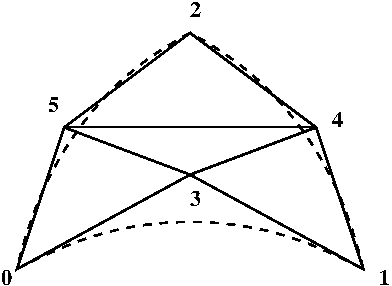
\includegraphics[width=0.55\textwidth]{bezier_images/q1.png} 
\end{figure}
\end{frame}

\begin{frame}{Measuring Quality}{A Curved Example}
The question is, {\bf if the linear triangle formed by the vertices has negative area, do I want to try and form a valid triangle}. \spa
I can think of this as taking a good triangle, and opening it up around a vertex until I have an invalid triangle from the vertices.
\begin{figure}
  \centering
  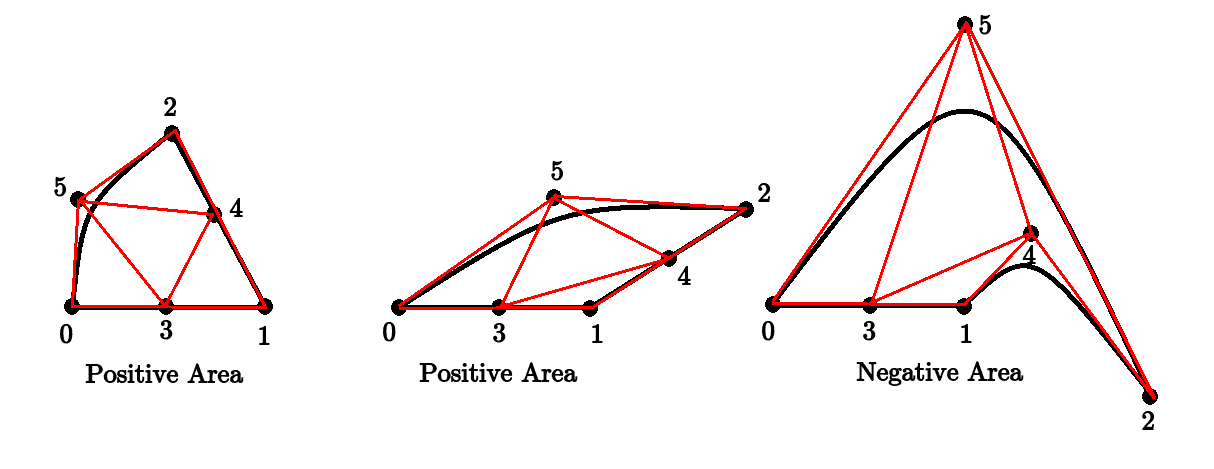
\includegraphics[width=0.95\textwidth]{bezier_images/q6.png} 
\end{figure}
We also have that for a triangle to have a negative linear area and be valid, that at least two edges must be curved.
\end{frame}

\begin{frame}{Measuring Quality}{A Curved Example}
Consider a simple three examples, with one edge linear between $(0,0)$ and $(1,0)$, and the other two allowed to curve, as in the canonical diagram shown earlier. \spa
Choose the remaining free vertex to be below the $x$-axis such that the vertices form a triangle with negative area. There are two free control points. \spa
These seem like a representative sample of triangles I could get if I allowed a negative linear area. I think they are all bad triangles. I could do a similar experiment for 3D, starting with one face linear, and allowing the others to curve...
\end{frame}
\begin{frame}{Measuring Quality}{A Curved Example}
Vertices are almost co-linear, but form a triangle with very small negative area.
\begin{figure}
  \centering
  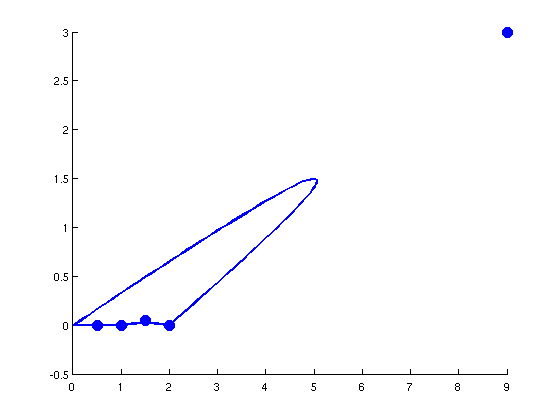
\includegraphics[width=0.60\textwidth]{bezier_images/curved1.png} 
\end{figure}
\[Q_l = -3\times 10^{-13}, Q_c = 0.013513, Q = -3\times10^{-15}\]
\end{frame}
\begin{frame}{Measuring Quality}{A Curved Example}
Control points chosen to maximize $Q_c$ but still maintain negative area, in this case, $Q_c \approx 1.$, but the element is very high aspect ratio.
\begin{figure}
  \centering
  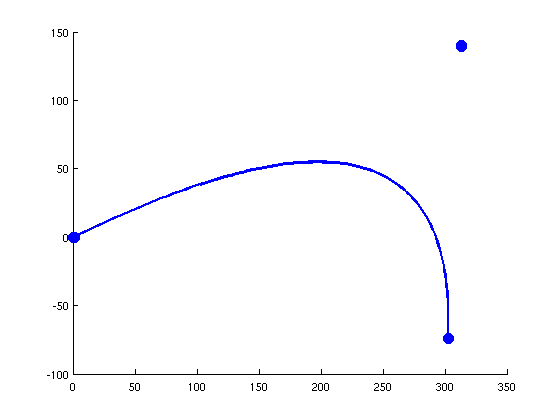
\includegraphics[width=0.60\textwidth]{bezier_images/curved2.png} 
\end{figure}
\[Q_l = -1.76\times10^{-6}, Q_c = 0.996, Q = -1.74\times10^{-6}\]
\end{frame}
\begin{frame}{Measuring Quality}{A Curved Example}
Control points chosen to maximize $Q$, both $Q_l$ and $Q_c$ are not horrible.
\begin{figure}
  \centering
  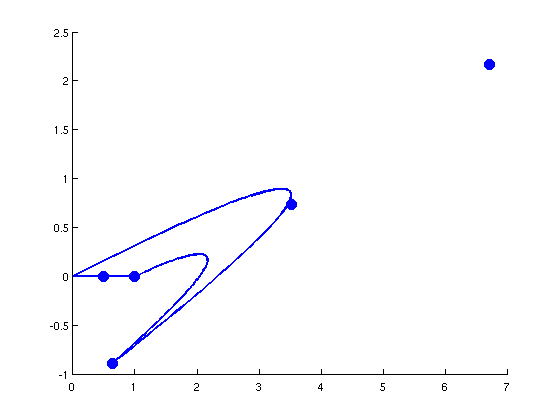
\includegraphics[width=0.60\textwidth]{bezier_images/curved3.png} 
\end{figure}
\[Q_l = -0.97 Q_c = 0.31, Q = -0.30\]
\end{frame}
\section{Determining Validity}
\begin{frame}{Determining Validity}
The convex hull property guarantees that if all control points of the Jacobian determinant are positive, the Jacobian determinant is positive everywhere, and thus the corresponding entity provably valid. For triangles (tetrahedra) the condition is
\[ N_{IJK(L)} > 0, \text{for all control points}\]
The contrary, however is not true. If one control point is negative, the Jacobian determinant is not necessarily negative everywhere, and thus the entity may be valid.\spa We use adaptive algorithms, converging the control points of the Jacobian determinant until we are confident of their sign.
\end{frame}
\begin{frame}{Determining Validity}
There are two approaches to adapting. \spa
1. {\bf Subdivision}. Any B{\'e}zier  can be split into multiple B{\'e}zier shapes that are identical to the original shape, with new control points.

2. {\bf Elevation}. Any B{\'e}zier shape can be elevated in order, preserving the original shape, with new control points. \spa

Since we have that the bounding shapes of B{\'e}zier shapes are themselves B{\'e}ziers, that is, the edges of a B{\'e}zier triangle are B{\'e}zier edges and so forth. This reduces the cost of the adaptive algorithm - e.g, if a coefficient of the Jacobian determinant on the edge is negative, we can simply adapt that edge repeatedly.
\end{frame}
\begin{frame}{Validity Check - Algorithm}
The algorithm is divided into two parts, a first screening, and a second, adaptive part ({\it The Generation of Valid Curvilinear Meshes}, Geuzaine et al.). \spa
The first part computes $\mathcal{J}$ at a prescribed set of $\mathbf{u}$, and if a negative value is found, the element is invalid. If all of these are positive, continue on to the adaptive part, to be sure. The adaptive part can use either elevation or subdivision.
\end{frame}
\begin{frame}{Validity Check - Initial}\scriptsize
\begin{algorithmic}[1]
\Function{CheckValidity}{entity}
\State compute $B_i$ for entity
\If{corner $B_i < 0$}
\State return INVALID, vertex(es) \Comment{Adaptation doesn't improve this}
\EndIf
\If{min $B_i > 0$} \Comment{may want $B_i > $ constant}
\State return VALID, empty 
\Else
\State find $B_i < 0$, determine edges, triangles to adapt
  \For{each lower entity to adapt}
    \State compute $B_i$ for that entity
    \If{CheckValidityAdaptive($B_{i,entity},\epsilon$,0) is \texttt{False}}
    \State entities $\gets$ entity
    \EndIf
  \EndFor
\EndIf
\If{entities is empty}
\State return VALID
\Else
\State return INVALID
\EndIf
\EndFunction
\end{algorithmic}
\end{frame}
\begin{frame}{Validity Check - Adaptive}\scriptsize
\begin{algorithmic}[1]
\Function{CheckValidityAdaptive}{$B_{i,entity},\epsilon$,nIter}
\If{min $B_i > 0$}
\State return VALID
\ElsIf{nIter $ > $ maxIter or change in min $B_i < \epsilon$}\Comment{Convergence check}
\State return INVALID
\Else
\State determine subdivisions or elevations
  \For{each entity in subdivisions or elevations}
  \State nIter $\gets$ nIter + 1
  \State checkValidityAdaptive($B_{i,entity},\epsilon$,nIter)
  \EndFor
\EndIf

\EndFunction
\end{algorithmic}
\end{frame}
\begin{frame}{Validity Check - Subdivision}
On subdivision, we can use either algorithm for subdivision, de Casteljau's algorithm or subdivision matrices. For tetrahedra, only subdivision matrices are implemented for the adaptive procedure. Both are implemented in the code, see \texttt{crv.h,crvQuality.cc}. It is not which one is faster. Convergence is determined if
\[
\max_i(|\min B_i^n - \min B_i^{n-1}|) < \epsilon
\]
\end{frame}
\begin{frame}{Validity Check - Elevation}
For elevation, we currently elevate by one order at a time, though this can easily be changed. \\

To determine when to this check is complete, either the maximum elevation order has been reached (in which case, $\min B_i$ is what it is), or the maximum total variation of the Jacobian determinant control points,
\[
\max_i |B_{i}-B_{i-1}| < \epsilon
\]
which is used to avoid early termination if simply $\max_i(|\min B_i^n - \min B_i^{n-1}|) < \epsilon$  as is used as in subdivision.
\end{frame}
\begin{frame}{Computing Jacobian Det Control Points}
There are two ways to compute $N_{IJK(L)}$, for example, in 3D, 
we could use the mathematical formulation of PL George (2014), which for computing each control point, is very expensive
{
  \footnotesize
\begin{eqnarray*}
N_{IJKL} = P^3 \displaystyle\sum_{|i|=I,|j|=J,|k|=K,|l|=L} \frac{{P-1 \choose i_1,j_1,k_1}{P-1 \choose i_2,j_2,k_2}{P-1 \choose i_3,j_3,k_3}}{ {3(P-1) \choose I,J,K}} \\  \times|\mathbf{C}_{i_1+1,j_1,k_1,l_1}-\mathbf{C}_{i_1,j_1+1,k_1,l_1},\\\mathbf{C}_{i_2+1,j_2,k_2,l_2}-\mathbf{C}_{i_2,j_2,k_2+1,l_2},\\
\mathbf{C}_{i_3+1,j_3,k_3,l_3}-\mathbf{C}_{i_3,j_3,k_3,l_3+1}|
\end{eqnarray*}
}

\end{frame}
\begin{frame}{Computing Jacobian Det Control Points}
Or we could use the approach of Remacle, and compute
\[
N = \mathbf{B}^{-1}\mathcal{J}
\]
where $\mathbf{B}^{-1}$ is the transformation matrix of order $3(P-1)$ and $\mathcal{J}$ is an vector containing the Jacobian determinants evaluated at the $\xi$ for the order $3(P-1)$ Bezier Shape. While computing the inverse of the matrix is expensive, when evaluating quality on a number of elements in a row, we can simply store this. I Believe this is faster for evaluating quality repeatedly, and worth investigating (both methods are implemented). \spa

This approach also works for all shapes, such as the blended shapes that are implemented.

\end{frame}
\section{Refinement}
\begin{frame}{Refinement}
Refinement is done using the subdivision principle of B{\'e}zier shapes. Consider the subdivision of a curve, creating a new curve from $\xi = a$ to $\xi = b$, $0 < a < b < 1$. Define $\xi_s = a+(b-a)\xi$, we can write the control points of the new curve, $\mathbf{C}_s$, in terms of the old curve as
\[
\mathbf{B}(\xi_s)\mathbf{C} = \mathbf{B}(\xi)\mathbf{C}_s
\]
The control points are then 
\[ 
\mathbf{C}_s = \mathbf{B}^{-1}\mathbf{B}_s \mathbf{C}
\]
With $\mathbf{B}_s = \mathbf{B}(\xi_s)$ and $\mathbf{B}^{-1}\mathbf{B}_s$ is the subdivision matrix for that particular subdivision.
\end{frame}
\begin{frame}{Refinement}
Using a subdivision matrix, we can determine control points for any new entity created from a split. Consider the 2-edge split of a cubic triangle. We want to determine the new control points for one of the edges, shown in red. In parametric space, it looks like this.
\begin{figure}
  \centering
  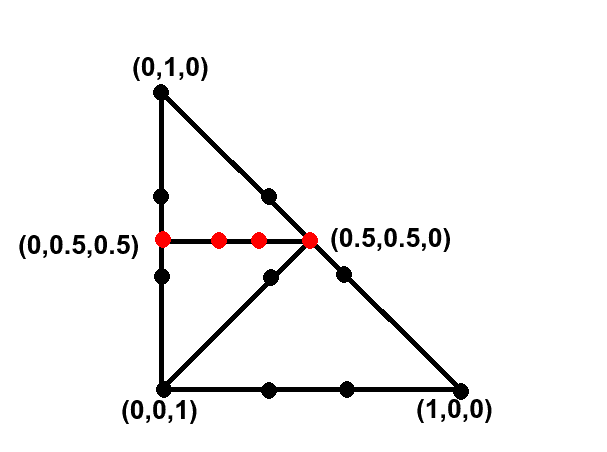
\includegraphics[width=0.55\textwidth]{bezier_images/refine1.png} 
\end{figure}
\end{frame}
\begin{frame}{Refinement}
To determine the control points on the edge between $a = (0,1/2,1/2)$ and $b = (1/2,1/2,0)$, we have \[\xi_s = (0,1/2,1/2), (1/2,1/2,0), (1/6,1/2,1/3), (1/3,1/2,1/6) \]
and the new control points as
\[ \mathbf{C}_s = \mathbf{B}^{-1}_{edge}\mathbf{B}_{triangle}(\xi_s) \mathbf{C} \]
where $\mathbf{B}_{edge}^{-1}$ is $4 \times 4$ and $\mathbf{B}_{triangle}(\xi_s)$ is $4 \times 9$ and $\mathbf{C}$ are the control points of the parent triangle. In practice, I don't solve for the endpoints, only the two control points on the edge. \spa
This approach can be used on every new entity created from the split and does not require apriori knowledge of the template used, only the parametric locations of the end points of the new entities.
\end{frame}
\begin{frame}{Refinement for Shape Correction}
As in the previous work, boundary edges are split if they form a 180$^\circ$ angle or more due to the geometry. This results in bad elements on the boundary. To overcome this, that edge should be split. If subdivision is used to perform the split, the invalidity is preserved. \spa To overcome this, new edges that connect to split edges are connected with linearly spaced points, and blending is used to place control points in triangles and tetrahedra created by the split.

\end{frame}
\begin{frame}{Refinement for Blended Shapes}
For blended shapes, a similar approach to mesh curving is used. The parametric locations of the new points on the parent are obtained, and interpolation points are then converted to control points to be used. 

\end{frame}
\section{Cavity Operations (Coarsening and Swapping)}
\begin{frame}{Cavity Problem For Curved Meshing}
Given a cavity of old elements ($d$ dimensional) and new entities, determine the control points on the new entities.
\begin{figure}
  \centering
  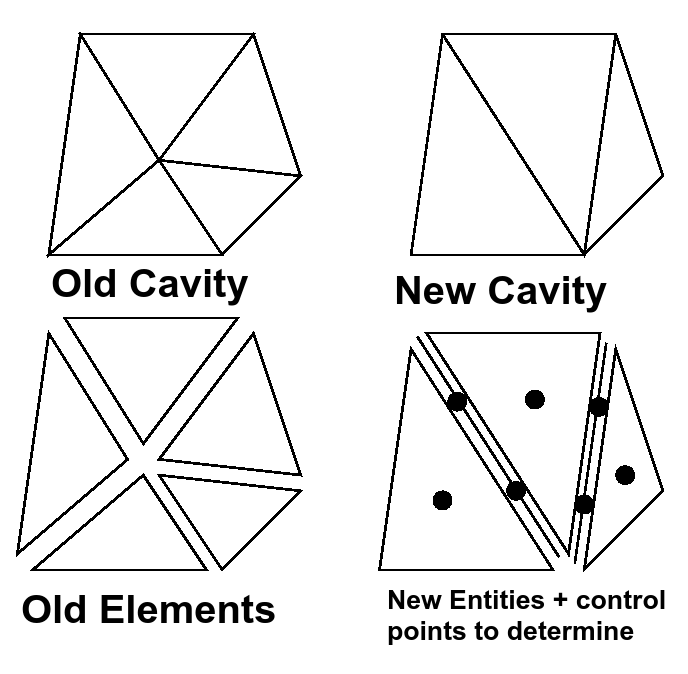
\includegraphics[width=0.45\textwidth]{bezier_images/cavity2.png} 
\end{figure}
In this 2D example with cubic mesh entities, there are 5 triangles in the old cavity, 3 triangles and 2 edges are newly created elements, and there are 7 control points to determine (2 on each new edge, 1 in each triangle).
\end{frame}

\begin{frame}{Edge Collapsing}
In the curved case, reconnecting with straight edges would result in an invalid mesh.
\begin{figure}
  \centering
  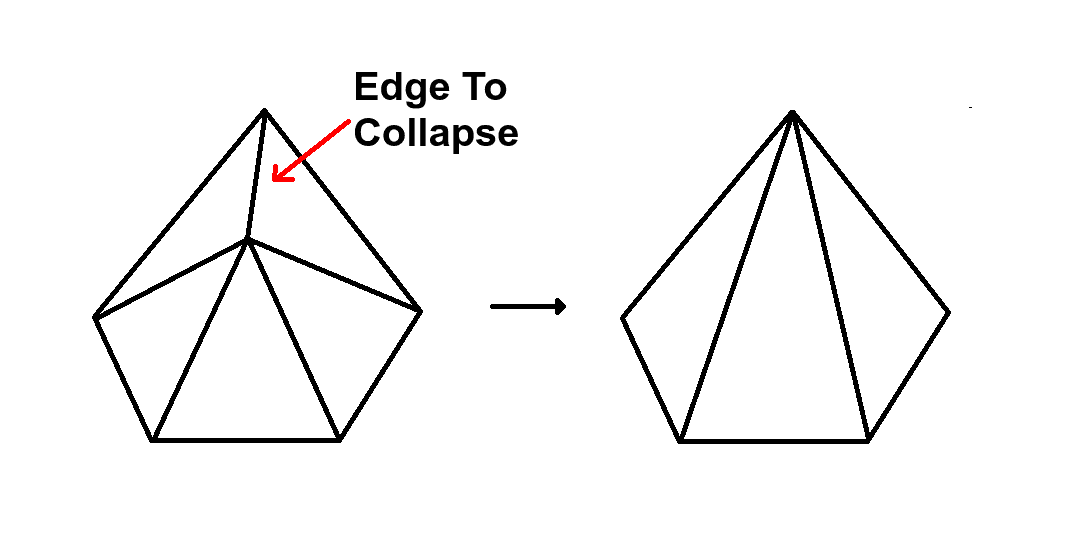
\includegraphics[width=0.55\textwidth]{bezier_images/collapse1.png} 
\end{figure}
\begin{figure}
  \centering
  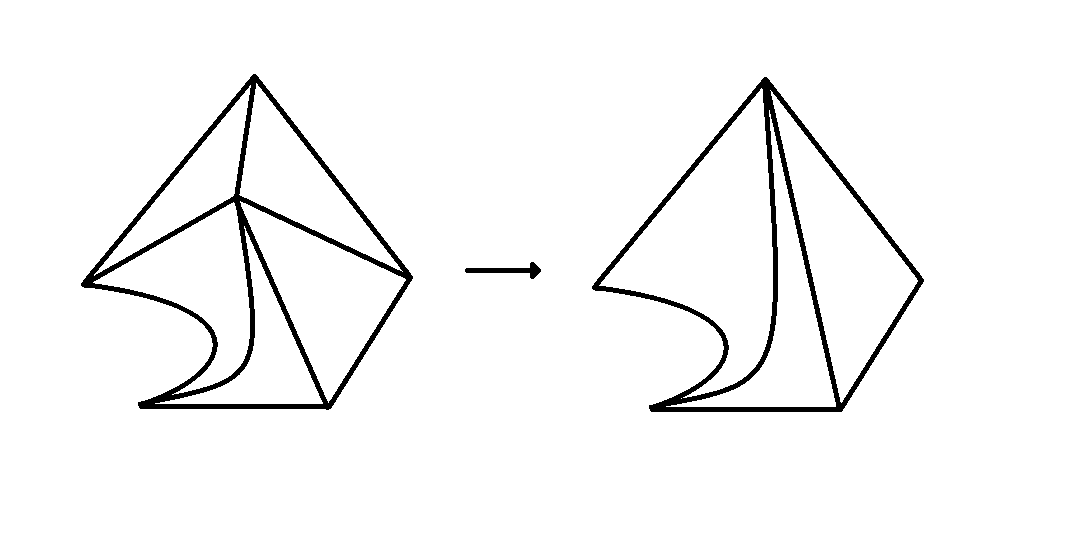
\includegraphics[width=0.55\textwidth]{bezier_images/collapse2.png} 
\end{figure}
\end{frame}

\begin{frame}{Edge Swapping}
\begin{figure}
  \centering
  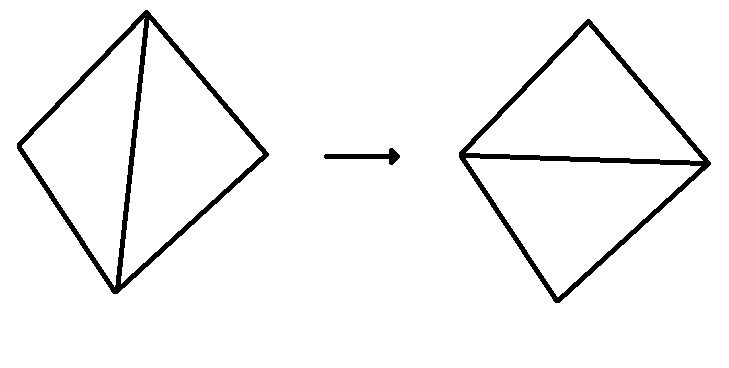
\includegraphics[width=0.45\textwidth]{bezier_images/swap1.png} 
\end{figure}
\begin{figure}
  \centering
  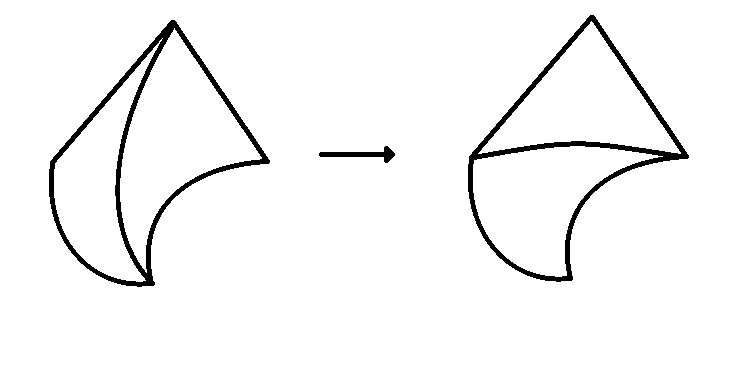
\includegraphics[width=0.45\textwidth]{bezier_images/swap2.png} 
\end{figure}
\end{frame}
\begin{frame}{Cavity Problem For Curved Meshing}
As the cavity connectivity is pre-determined by the linear configurations, and the problem is to find a path within the cavity that does not intersect the sides of the cavity.
\begin{figure}
  \centering
  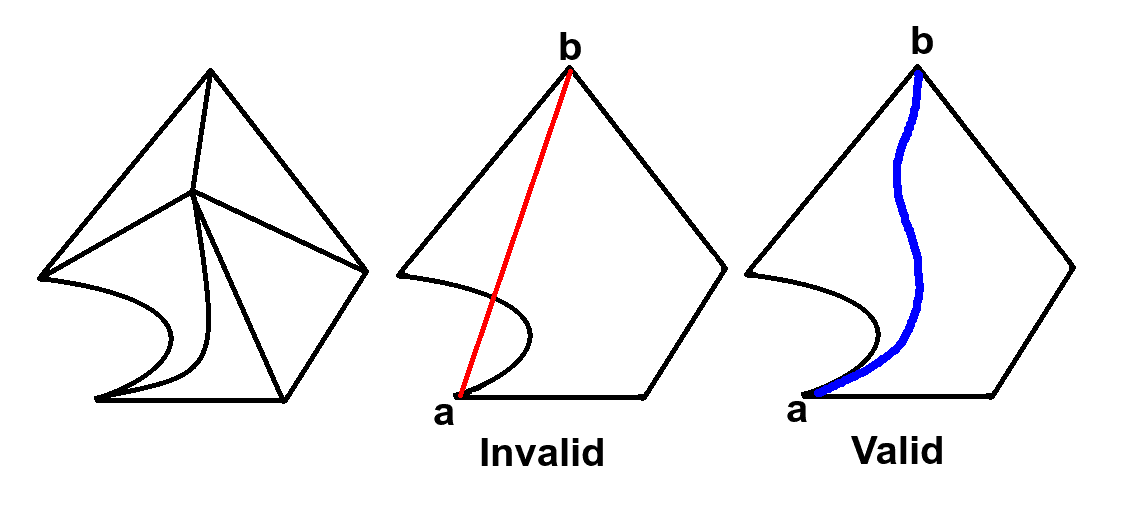
\includegraphics[width=0.65\textwidth]{bezier_images/collapse4.png} 
\end{figure}
Once the edge control points are chosen, the triangle control points can be determined using a blending of the edge points (serendipity-like approach), thus for now, only the edge control points are of interest.
\end{frame}
\begin{frame}{Previous Approaches}
\textit{Automatic p-version mesh generation for curved domains}, SCOREC 
\begin{figure}
  \centering
  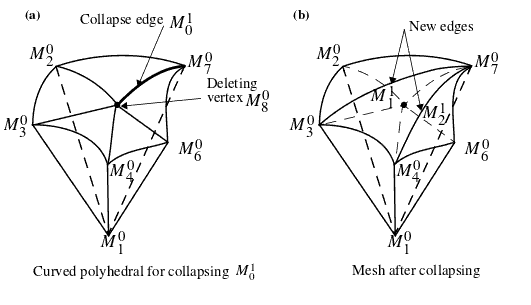
\includegraphics[width=0.75\textwidth]{bezier_images/collapseOld2.png} 
\end{figure}
Edges placed based on forming a quadrilateral around the edge and blending
\end{frame}
\begin{frame}{Previous Approaches}
\textit{Automatic p-version mesh generation for curved domains}, SCOREC
\begin{figure}
  \centering
  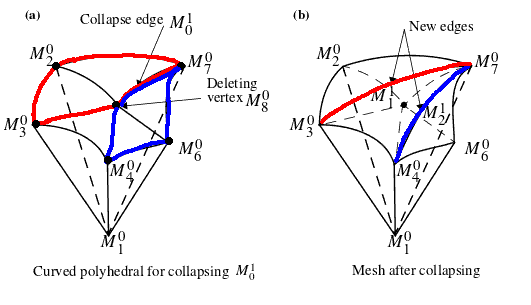
\includegraphics[width=0.75\textwidth]{bezier_images/collapseOld3.png} 
\end{figure}
Quadrilaterals for the two edges shown here, and blending is formed. 
\end{frame}
\begin{frame}{Previous Approaches}
\textit{Automatic p-version mesh generation for curved domains}, SCOREC \spa
Quadrilaterals to blend are shown here, with new edge.
\begin{figure}
  \centering
  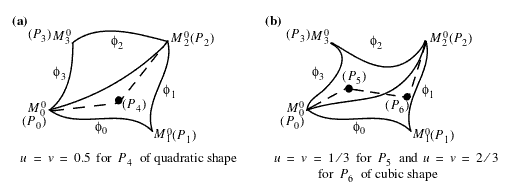
\includegraphics[width=0.75\textwidth]{bezier_images/collapseOld4.png} 
\end{figure}
2nd and 3rd orders are shown here. for higher than 3rd, we can either elevate the third, or just use equally spaced points.
\end{frame}
\begin{frame}{Previous Approaches}
\textit{Automatic p-version mesh generation for curved domains}, SCOREC \spa
Quadrilaterals to blend are shown here, with new edge.
\begin{figure}
  \centering
  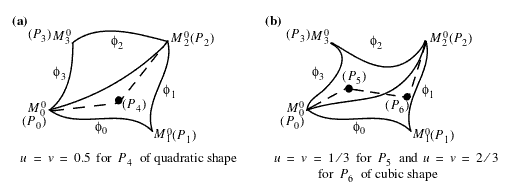
\includegraphics[width=0.75\textwidth]{bezier_images/collapseOld4.png} 
\end{figure}
Requires collecting and orienting edges, still no guarantees the blended edge creates valid elements. Using the notation in the paper the equation is
{\footnotesize
\begin{eqnarray*}
x = (1-v)\phi_0(u)+u\phi_1(v)+v\phi_2(1-u)+(1-u)\phi_3(1-v) \\
- (1-u)(1-v)P_0 - (1-v)uP_1 - uvP_2 -(1-u)vP_3 
\end{eqnarray*}
}
\end{frame}
\begin{frame}{Quad Blending}
 One downside to this approach is that it will result in curving edges unnecessarily, e.g. in the swap,
\begin{figure}
  \centering
  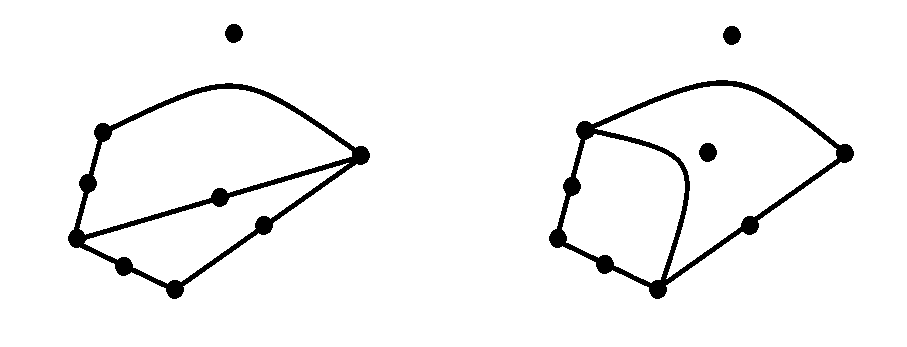
\includegraphics[width=0.75\textwidth]{bezier_images/swap3.png} 
\end{figure}
the new edge could (and I think should) be straight.
\end{frame}
\begin{frame}{Quad Blending - 2D Collapses}
While this approach is described as a 3D approach, it still raises some questions which are not addressed in the literature. For example, looking at the 2D problem, consider a collapse with 6 triangles in the cavity.
\begin{figure}
  \centering
  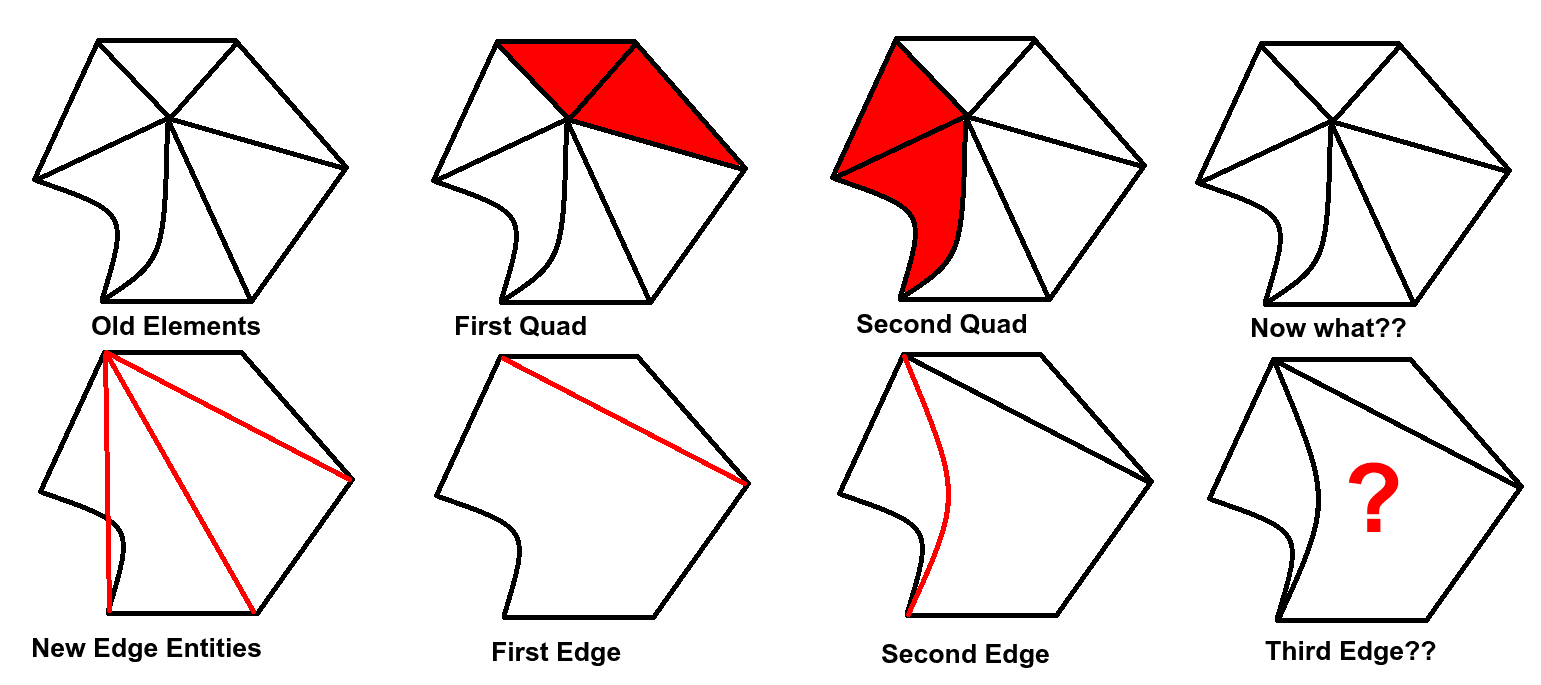
\includegraphics[width=0.75\textwidth]{bezier_images/collapse9.png} 
\end{figure}
How do we determine the middle edge?
\end{frame}
\begin{frame}{Quad Blending - 2D Collapses}
In this case, its fairly easy to see how we can use the first two edges to determine the middle edge.
\begin{figure}
  \centering
  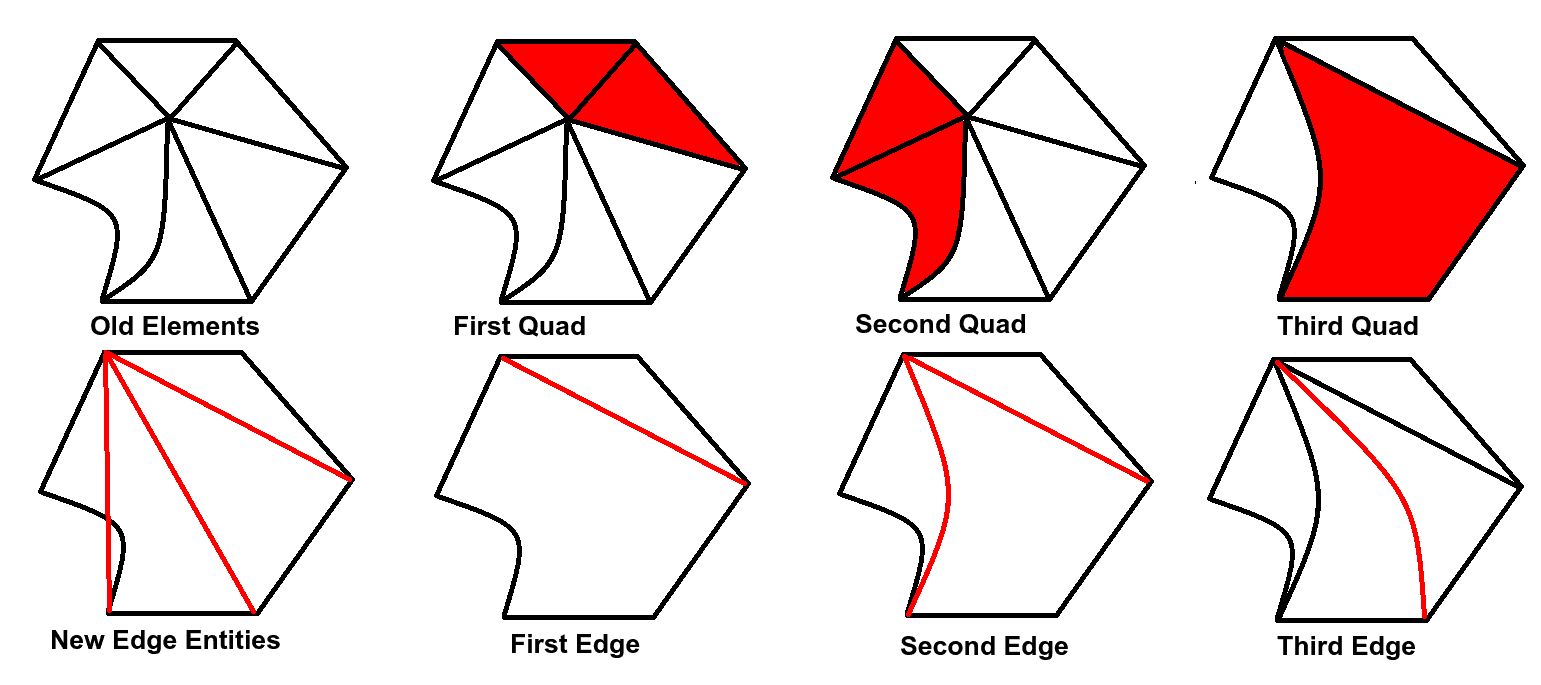
\includegraphics[width=0.75\textwidth]{bezier_images/collapse10.png} 
\end{figure}

\end{frame}
\begin{frame}{Quad Blending - 2D Collapses}
But now what happens if we have 7 (or more) triangles in the collapse?
\begin{figure}
  \centering
  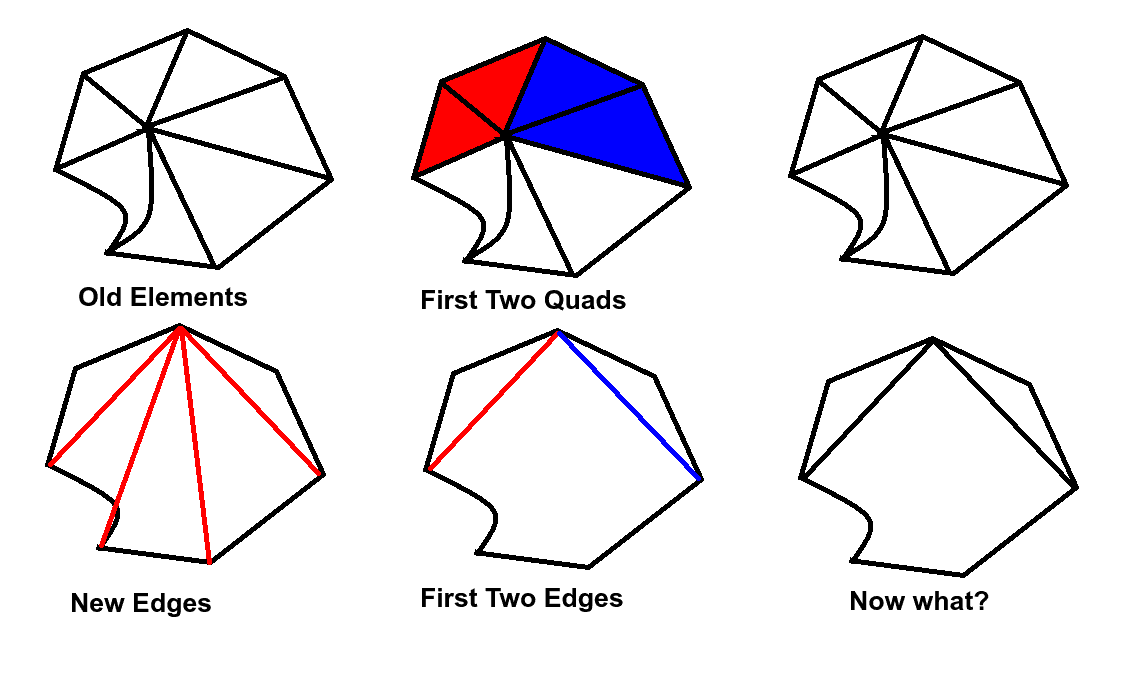
\includegraphics[width=0.75\textwidth]{bezier_images/collapse11.png} 
\end{figure}
We have a choice to make.  We can assume one is linear and solve for the other, as shown on the next slide.
\end{frame}
\begin{frame}{Quad Blending - 2D Collapses}
But now what happens if we have 7 (or more) triangles in the collapse?
\begin{figure}
  \centering
  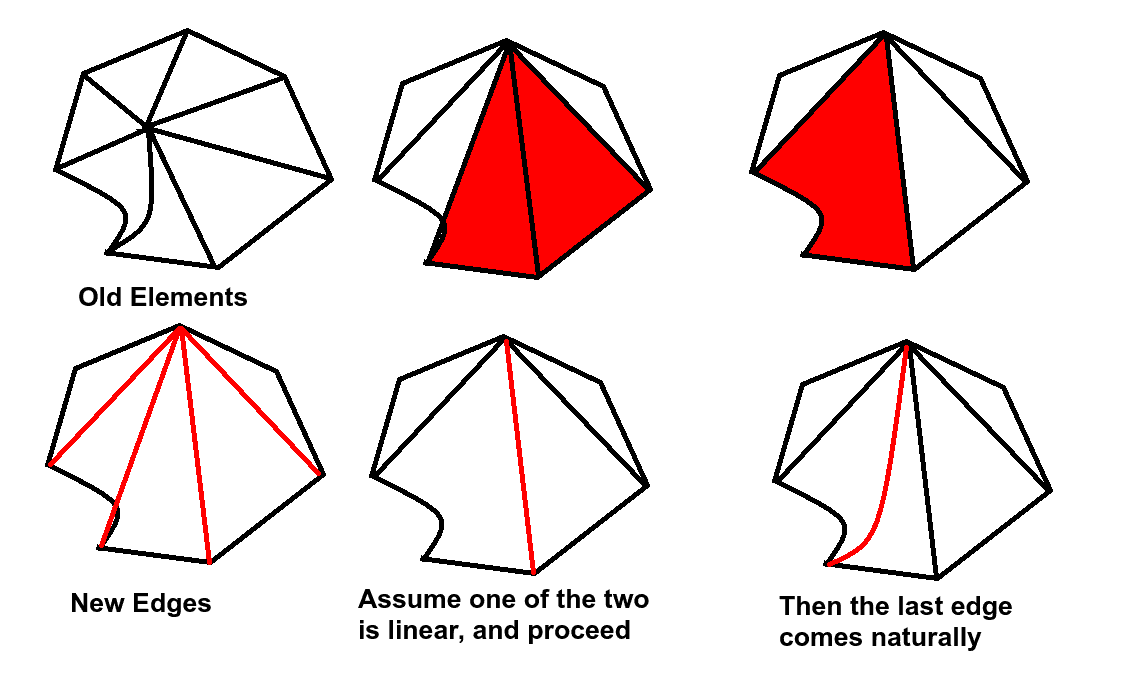
\includegraphics[width=0.75\textwidth]{bezier_images/collapse12.png} 
\end{figure}
In this case, currently straight lines are assumed for the middle edges, nothing smarter is done.
\end{frame}

\begin{frame}{Quad Blending - 3D Collapses}
Collapses are similar in 3D, for example, shown below, we have two quads we can form, and the new edges form naturally.
\begin{figure}
  \centering
  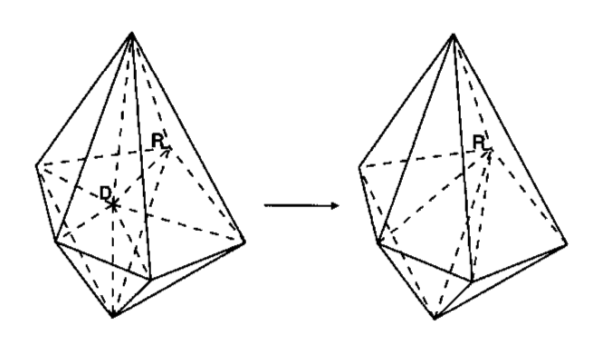
\includegraphics[width=0.65\textwidth]{bezier_images/edgeCollapse.png} 
\end{figure}
This is largely because of the diagram itself, in reality
\end{frame}
\begin{frame}{Quad Blending - 3D Collapses}
Collapses are similar in 3D, for example, shown below, we have two quads we can form, one for each edge, and the new edges form naturally.
\begin{figure}
  \centering
  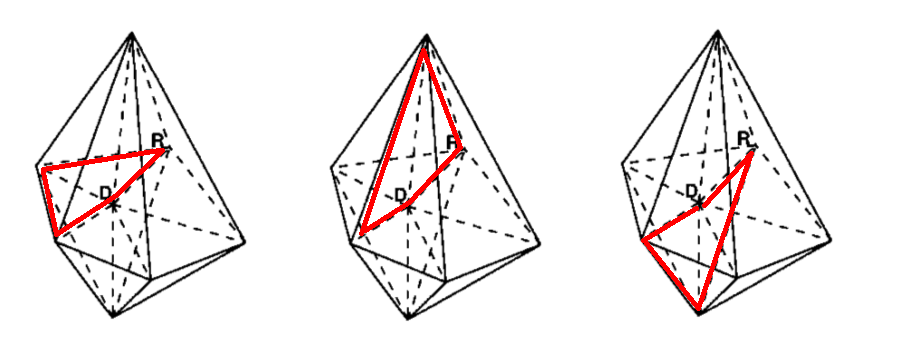
\includegraphics[width=0.65\textwidth]{bezier_images/edgeCollapse3.png} 
\end{figure}
This is largely because of the way the diagram is drawn, in reality, there are three quads we could choose for the left edge. In this case, the quadrilateral with the smallest "linear" area is chosen, and they are blended, on the idea that they are most likely to influence the new edge.
\end{frame}

\begin{frame}{Quad Blending - 3D Collapses}
In the same diagram, if we had collapsed to the bottom vertex, there are 5 quads we could have chosen.
\begin{figure}
  \centering
  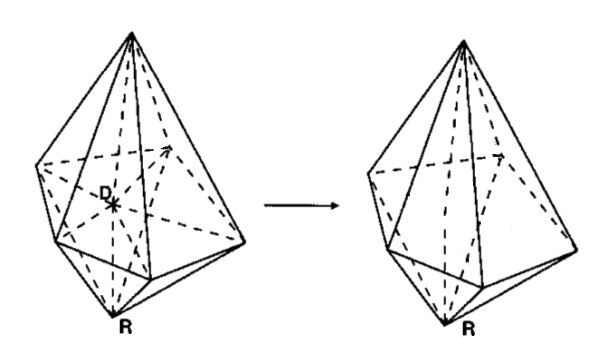
\includegraphics[width=0.65\textwidth]{bezier_images/edgeCollapse2.png} 
\end{figure}
Which one should be chosen?
\end{frame}
\begin{frame}{Quad Blending - 3D Swaps}
We note that the new entities shown in the previous cases are the new entities present from a 3D edge swap (with the edge connecting a top/bottom vertices swapped out). \spa For all edge swaps, there is no single pair of triangles to blend into a quad. For an interior swap, all new edges formed connect with four triangles (two in the ring, one with each vertex of the original edge).
\begin{figure}
  \centering
  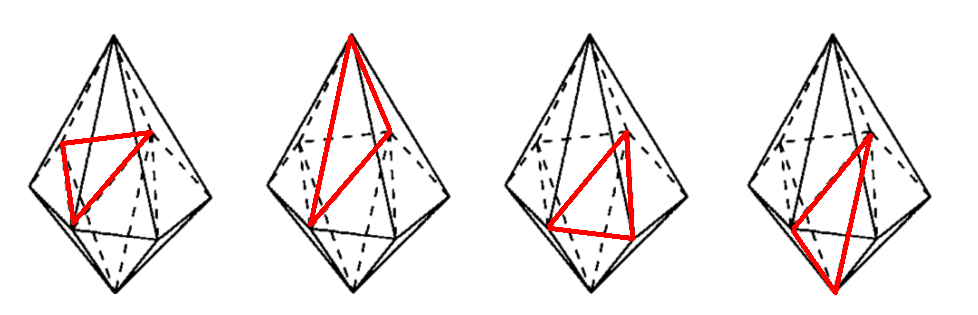
\includegraphics[width=0.65\textwidth]{bezier_images/edgeSwap.png} 
\end{figure}
\end{frame}
\begin{frame}{Quad Blending - 3D Swaps}
With four triangles to choose from, we have a choice to make. We could blend the two triangles in the ring, however it is easy to construct an example where those four edges are less influential than those of another pair of edges. In this case, the pair of triangles with the smallest "linear" area is chosen, and they are blended, on the idea that they are most likely to influence the new edge.
\begin{figure}
  \centering
  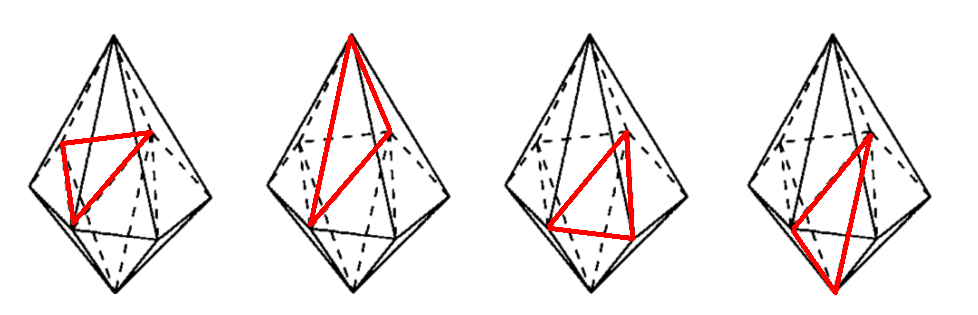
\includegraphics[width=0.65\textwidth]{bezier_images/edgeSwap.png} 
\end{figure}
\end{frame}
\begin{frame}{Coarsening and Swapping for Blended Shapes}
For blended shapes, as only edge placement matters, this is fairly trivial. Whether the blending is valid is a different story, but nonetheless, once edge node placement is decided, we are done.

\end{frame}
\section{Curved Adaptation and Shape Correction}

\begin{frame}{Curved Adaptation and Shape Correction}{\textit{Automatic p-version mesh generation for curved domains} (XJ Luo et al, 2004)}
Curved adaptation and shape correction are implemented in \texttt{crvAdapt.cc}. First, a pass of shape correction to attempt to fix invalid elements is performed, followed by the normal adaptive loop with refinement and coarsening to match length scales. This is followed by another pass of shape correction. Shape correction is implemented as, in increasing order of cost.\spa
While the number of invalid elements is decreasing:
\begin{enumerate}
\item Fix Large Boundary Angles by splitting
\item If is second-order, reposition mid edge nodes (shown a few slides from now)
\item Collapse Invalid Edges
\item Swap Invalid Edges
\end{enumerate}
\end{frame}
\begin{frame}{Curved Adaptation and Shape Correction}

In each case, the operation is only performed if it makes elements valid. Going from bad quality (invalid, < 0), to better quality but still invalid is not done. In practice, this may actually help gradually improve things, but right now, this is not the implementation. \spa
To determine which edges to mark, the validity of an element is used.
\end{frame}
\begin{frame}{Curved Adaptation and Shape Correction}

If an element is invalid at a vertex, the connecting edges are marked.\\
If an element is invalid at an edge, that edge is marked. \\
If an element is invalid on a face, that faces edges are marked.\\
If an element is invalid on its interior, all its edges are marked.\\
In each case, only the first invalidity is marked. If an element is invalid in multiple places, only one of them will be flagged.
\end{frame}
\begin{frame}{Mid-edge Node Repositioning}
This is exactly as in the work in XJ Luo's thesis. This is implemented in \texttt{crvReposition.cc}. Given a tetrahedron and an edge marked as invalid, one of the edges' two vertices are used for repositioning. In this implementation, the edge with the worse jacobian determininant is chosen (one of them must be negative, choose the more negative one). \spa
Denote the vector connecting the invalid edge's midpoint node to the vertex as $\mathbf{a}$, and the other two vectors connected edges to the chosen vertex as $\mathbf{b}$ and $\mathbf{c}$. For the invalidity, we have that $\mathbf{a}\cdot (\mathbf{b}\times\mathbf{c}) < 0$. To correct it, we need to choose $\mathbf{a}$ such that this is positive.
\end{frame}
\begin{frame}{Mid-edge Node Repositioning} 
Denote the new vector as $\mathbf{a}'$ 
\[
\mathbf{a}' = \frac{\mathbf{n}}{||\mathbf{n}||}(-\frac{\mathbf{a}\cdot \mathbf{n}}{||\mathbf{n}||} + ||\mathbf{a}||\sin(\theta)
\]
where $\mathbf{n} = \mathbf{b}\times\mathbf{c} $ and $\theta$ is the angle between $\mathbf{a}'$ and the plane defined by $\mathbf{n}$ and the chosen vertex. This places the new point on the other side of this plane, hopefully creating a valid element. If all the elements adjacent to the modified edge are valid, the operation is accepted and the invalid element has been fixed.
\end{frame}
\section{$G^1$ Continuous Patches}
\begin{frame}{$G^1$ Continuous Patches}
G1 continuous patches are implemented following Walton and Meek, \textit{A triangular G1 patch from boundary curves}. The mesh is initially set to 4th order, with 6 face nodes for the G1 patch. First, all edges on a geometric surface have control points set (the first two nodes of the three) using surface normals and the vertex locations. Edges on geometric edges have their control points set using the tangents at their endpoints. These edge control points use the algorithm of Walton and Meek to set the six face nodes. Once the internal points are determined, the edges are formally elevated, by resetting all of the points to the elevated control points.
\end{frame}
\begin{frame}{$G^1$ Continuous Patches}
The weights on these nodes are similar to the triangular B{\'e}zier, with the evaluation done as if it is a B{\'e}zier triangle with internal B{\'e}zier points, $\mathbf{B}$, and Gregory points, $\mathbf{G}$.
\begin{equation}
\mathbf{B}_{12} = \frac{1}{\xi_1+\xi_2}(\xi_2\mathbf{G}_{12}+\xi_1\mathbf{G}_{17})
\end{equation}
\begin{equation}
\mathbf{B}_{13} = \frac{1}{\xi_0+\xi_2}(\xi_0\mathbf{G}_{13}+\xi_2\mathbf{G}_{15})
\end{equation}
\begin{equation}
\mathbf{B}_{14} = \frac{1}{\xi_0+\xi_1}(\xi_1\mathbf{G}_{14}+\xi_0\mathbf{G}_{16})
\end{equation}
The remainder of the mathematics is the same as the B{\'e}zier triangle, with tetrahedral blending, and other aspects maintaining the same form. We should note that choosing $\mathbf{G}_{12} = \mathbf{G}_{17}, \mathbf{G}_{13} = \mathbf{G}_{15}, \mathbf{G}_{14} = \mathbf{G}_{16}$ results in the original B{\'e}zier triangle, albeit with three additional nodes stored per triangle.
\end{frame}
\begin{frame}{$G^1$ Continuous Patches}
\begin{figure}
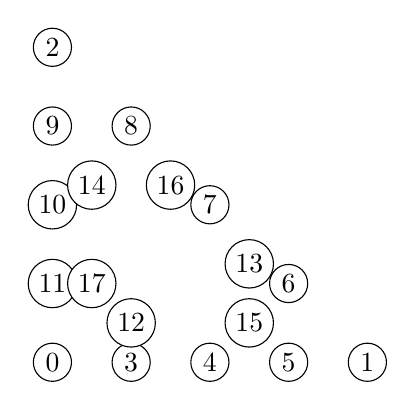
\begin{tikzpicture}[scale=1]
\tikzstyle{every node}=[circle, draw, fill=white,
                        inner sep=2pt, minimum width=5pt]
\path (0,0) node {$0$}
(1,0) node {$3$}
(2,0) node {$4$}
(3,0) node {$5$}
(4,0) node {$1$}
(3,1) node {$6$}
(2,2) node {$7$}
(1,3) node {$8$}
(0,4) node {$2$}
(0,3) node {$9$}
(0,2) node {$10$}
(0,1) node {$11$}
(1.0,0.5) node {$12$}
(2.5,1.25) node {$13$}
(0.5,2.25) node {$14$}
(2.5,0.5) node {$15$}
(1.5,2.25) node {$16$}
(0.5,1.0) node {$17$};

\end{tikzpicture} \hspace{0.5cm}
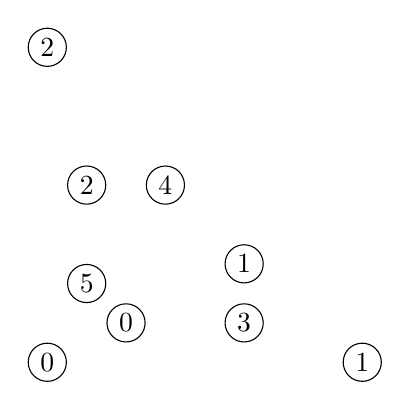
\begin{tikzpicture}[scale=1]
\tikzstyle{every node}=[circle, draw, fill=white,
                        inner sep=2pt, minimum width=5pt]
\path (0,0) node {$0$}

(4,0) node {$1$}

(0,4) node {$2$}

(1.0,0.5) node {$0$}
(2.5,1.25) node {$1$}
(0.5,2.25) node {$2$}
(2.5,0.5) node {$3$}
(1.5,2.25) node {$4$}
(0.5,1.0) node {$5$};

\end{tikzpicture}
\end{figure}
Global and local node ordering for the 4th order G1 triangle. The ordering is chosen as these points are set based on edges, so node 0 and node 3 correspond to edge 0 and so forth.
\end{frame}
\section{Implementation}
\begin{frame}{Parametrization - Curves}
For curves, there is one free parameter, $u$ (v = 1-u), between 0 and 1. In finite element convention, the parameter, $\xi \in [-1,1]$, such that
\[ u = \frac{1}{2}(\xi+1)\]
When taking derivatives we have that
\[ \frac{\mathrm{d} \mathbf{B}(u)}{\mathrm{d} \xi}  =  \frac{\mathrm{d} \mathbf{B}(u)}{\mathrm{d} u}\frac{\mathrm{d} u}{\mathrm{d} \xi} = \frac{1}{2}\frac{\mathrm{d} \mathbf{B}(u)}{\mathrm{d} u}
\]

\end{frame}
\begin{frame}{Parametrization - Triangles}
For triangles, there are two free parameters, $u,v,(w = 1-u-v)$, between 0 and 1. In finite element convention, the parameters, $\xi_0,\xi_1 \in [0,1]$, are such that 
$\xi_0 = 1$, corresponds to vertex 1, $\xi_1 = 1$ to vertex 2, such that the barycentric coordinates are
\[(u,v,w) = (1-\xi_0-\xi_1,\xi_0,\xi_1)\]
When taking derivatives, writing $\mathbf{B}(\xi_0,\xi_1) = \mathbf{B}(u,v,w)$
{
  \footnotesize
\[ \frac{\mathrm{d} \mathbf{B}}{\mathrm{d} \xi_0}  =  \frac{\mathrm{d} \mathbf{B}}{\mathrm{d} u}\frac{\mathrm{d} u}{\mathrm{d} \xi_0} + \frac{\mathrm{d} \mathbf{B}}{\mathrm{d} v}\frac{\mathrm{d} v}{\mathrm{d} \xi_0} = -\frac{\mathrm{d} \mathbf{B}}{\mathrm{d} u}+\frac{\mathrm{d} \mathbf{B}}{\mathrm{d} v}
\]
\[ \frac{\mathrm{d} \mathbf{B}}{\mathrm{d} \xi_1} = -\frac{\mathrm{d} \mathbf{B}}{\mathrm{d} u}+\frac{\mathrm{d} \mathbf{B}}{\mathrm{d} w}
\]
}
\end{frame}
\begin{frame}{Parametrization - Tetrahedra}
For tetrahedra, there are three free parameters, $u,v,w,(t = 1-u-v-w)$, between 0 and 1. In finite element convention, the parameters, $\xi_0,\xi_1,\xi_2 \in [0,1]$
\[(u,v,w,t) = (1-\xi_0-\xi_1-\xi_2,\xi_0,\xi_1,\xi_2)\]
When taking derivatives we have that, similar to triangles,
{
  \footnotesize
\[ \frac{\mathrm{d} \mathbf{B}}{\mathrm{d} \xi_0}  =  \frac{\mathrm{d} \mathbf{B}}{\mathrm{d} u}\frac{\mathrm{d} u}{\mathrm{d} \xi_0} + \frac{\mathrm{d} \mathbf{B}}{\mathrm{d} v}\frac{\mathrm{d} v}{\mathrm{d} \xi_0} + \frac{\mathrm{d} \mathbf{B}}{\mathrm{d} w}\frac{\mathrm{d} w}{\mathrm{d} \xi_0}+ \frac{\mathrm{d} \mathbf{B}}{\mathrm{d} w}\frac{\mathrm{d} t}{\mathrm{d} \xi_0} = -\frac{\mathrm{d} \mathbf{B}}{\mathrm{d} u}+\frac{\mathrm{d} \mathbf{B}}{\mathrm{d} v}
\]
\[ \frac{\mathrm{d} \mathbf{B}}{\mathrm{d} \xi_1} = -\frac{\mathrm{d} \mathbf{B}}{\mathrm{d} u}+\frac{\mathrm{d} \mathbf{B}}{\mathrm{d} w} 
\]
\[ \frac{\mathrm{d} \mathbf{B}}{\mathrm{d} \xi_2} = -\frac{\mathrm{d} \mathbf{B}}{\mathrm{d} u}+\frac{\mathrm{d} \mathbf{B}}{\mathrm{d} t}
\]
}
\end{frame}
\begin{frame}{Ordering}
All ordering is in \texttt{crvTables.cc}. For triangles 10th order and below and tetrahedra 6th order and below, the ordering is stored in tables. Otherwise, it is computed as needed. 
\end{frame}
\begin{frame}{Ordering - Curves}
Due to shared entities, there is a specific order to store coordinates in a 1D Array. This ordering is used in \texttt{apfShape.h} and nodes from \texttt{apf::getVectorNodes} return the coordinates in this specific ordering. The ordering is stored in \texttt{crvTables.cc}, e.g for triangles in \texttt{getTriNodeIndex(P,i,j)}. \spa

For curves, this is simple. The vertex control points are indexed into 0 and 1, with the remaining points ordered as in the figure below, for a third order curve.
\begin{figure}
\centering
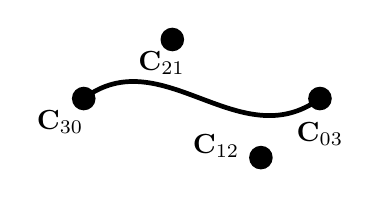
\begin{tikzpicture}[scale=3.0] 
\draw [line width=0.6mm, black ] (0, 0) .. controls (0.33,0.25) and (0.66,-0.25)
   .. (1.0, 0.);
\path (-0.1,-0.1) node {$\mathbf{C}_{30}$}
(0.33,0.15) node {$\mathbf{C}_{21}$}
(0.56,-0.2) node {$\mathbf{C}_{12}$}
(1.0,-0.15) node {$\mathbf{C}_{03}$};

\fill (0,0) circle [radius=0.5mm];
\fill (0.375,0.25) circle [radius=0.5mm];
\fill (.75,-.25) circle [radius=0.5mm];
\fill (1.,0) circle [radius=0.5mm];
\end{tikzpicture}
\hspace{1cm}
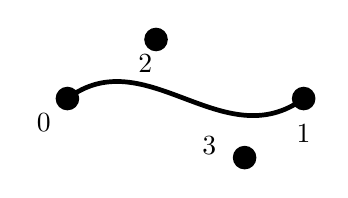
\begin{tikzpicture}[scale=3.0] 
\draw [line width=0.6mm, black ] (0, 0) .. controls (0.33,0.25) and (0.66,-0.25)
   .. (1.0, 0.);
\path (-0.1,-0.1) node {$0$}
(0.33,0.15) node {$2$}
(0.60,-0.2) node {$3$}
(1.0,-0.15) node {$1$};

\fill (0,0) circle [radius=0.5mm];
\fill (0.375,0.25) circle [radius=0.5mm];
\fill (.75,-.25) circle [radius=0.5mm];
\fill (1.,0) circle [radius=0.5mm];
\end{tikzpicture}
\end{figure}
\end{frame}
\begin{frame}{Ordering - Triangles}
For triangles, this is more complex. The vertices come first, followed by the edge control points, followed by the triangle's internal points.
\begin{figure}
\centering
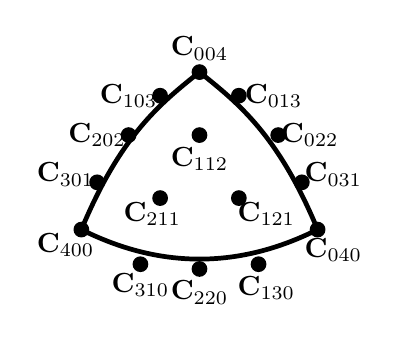
\begin{tikzpicture}[scale=2.0] 
\draw [line width=0.6mm, black ] (0, 0) .. controls (0.5,-0.25) and (1.0, -0.25)
   .. (1.5, 0.) .. controls (1.25,0.6) and (1.0,0.8) 
   .. (0.75,1.) .. controls (0.5,0.8) and (0.25,0.6) 
   .. (0,0); 

\path (-0.1,-0.1) node {$\mathbf{C}_{400}$}
(0.375,-0.35) node {$\mathbf{C}_{310}$}
(0.75,-0.4) node {$\mathbf{C}_{220}$}
(1.175,-0.37) node {$\mathbf{C}_{130}$}
(1.6,-0.13) node {$\mathbf{C}_{040}$}
(1.6,0.35) node {$\mathbf{C}_{031}$}
(1.45,0.6) node {$\mathbf{C}_{022}$}
(1.22,0.85) node {$\mathbf{C}_{013}$}
(0.75,1.15) node {$\mathbf{C}_{004}$}
(-0.1,0.35) node {$\mathbf{C}_{301}$}
(0.1,0.6) node {$\mathbf{C}_{202}$}
(0.3,0.85) node {$\mathbf{C}_{103}$}
(0.45,0.1) node {$\mathbf{C}_{211}$}
(1.175,0.1) node {$\mathbf{C}_{121}$}
(0.75,0.45) node {$\mathbf{C}_{112}$};
\fill (0,0) circle [radius=0.5mm];
\fill (0.375,-0.22) circle [radius=0.5mm];
\fill (.75,-.25) circle [radius=0.5mm];
\fill (1.125,-.22) circle [radius=0.5mm];
\fill (1.5,0) circle [radius=0.5mm];
\fill (1.4,0.3) circle [radius=0.5mm];
\fill (1.25,0.6) circle [radius=0.5mm];
\fill (1.0,0.85) circle [radius=0.5mm];
\fill (0.1,0.3) circle [radius=0.5mm];
\fill (0.3,0.6) circle [radius=0.5mm];
\fill (0.5,0.85) circle [radius=0.5mm];
\fill (0.5,0.2) circle [radius=0.5mm];
\fill (1.0,0.2) circle [radius=0.5mm];
\fill (0.75,0.6) circle [radius=0.5mm];
\fill (0.75,1.) circle [radius=0.5mm];
\end{tikzpicture} 
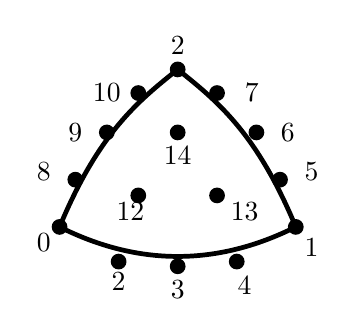
\begin{tikzpicture}[scale=2.0] 
\draw [line width=0.6mm, black ] (0, 0) .. controls (0.5,-0.25) and (1.0, -0.25)
   .. (1.5, 0.) .. controls (1.25,0.6) and (1.0,0.8) 
   .. (0.75,1.) .. controls (0.5,0.8) and (0.25,0.6) 
   .. (0,0); 

\path (-0.1,-0.1) node {$0$}
(0.375,-0.35) node {$2$}
(0.75,-0.4) node {$3$}
(1.175,-0.37) node {$4$}
(1.6,-0.13) node {$1$}
(1.6,0.35) node {$5$}
(1.45,0.6) node {$6$}
(1.22,0.85) node {$7$}
(0.75,1.15) node {$2$}
(-0.1,0.35) node {$8$}
(0.1,0.6) node {$9$}
(0.3,0.85) node {$10$}
(0.45,0.1) node {$12$}
(1.175,0.1) node {$13$}
(0.75,0.45) node {$14$};
\fill (0,0) circle [radius=0.5mm];
\fill (0.375,-0.22) circle [radius=0.5mm];
\fill (.75,-.25) circle [radius=0.5mm];
\fill (1.125,-.22) circle [radius=0.5mm];
\fill (1.5,0) circle [radius=0.5mm];
\fill (1.4,0.3) circle [radius=0.5mm];
\fill (1.25,0.6) circle [radius=0.5mm];
\fill (1.0,0.85) circle [radius=0.5mm];
\fill (0.1,0.3) circle [radius=0.5mm];
\fill (0.3,0.6) circle [radius=0.5mm];
\fill (0.5,0.85) circle [radius=0.5mm];
\fill (0.5,0.2) circle [radius=0.5mm];
\fill (1.0,0.2) circle [radius=0.5mm];
\fill (0.75,0.6) circle [radius=0.5mm];
\fill (0.75,1.) circle [radius=0.5mm];
\end{tikzpicture}
\end{figure}
\end{frame}
\begin{frame}{Ordering - Triangles}
On the interior, the points are ordered in a zig zag pattern, e.g for a $5^{th}$ order triangle
\begin{figure}
\centering
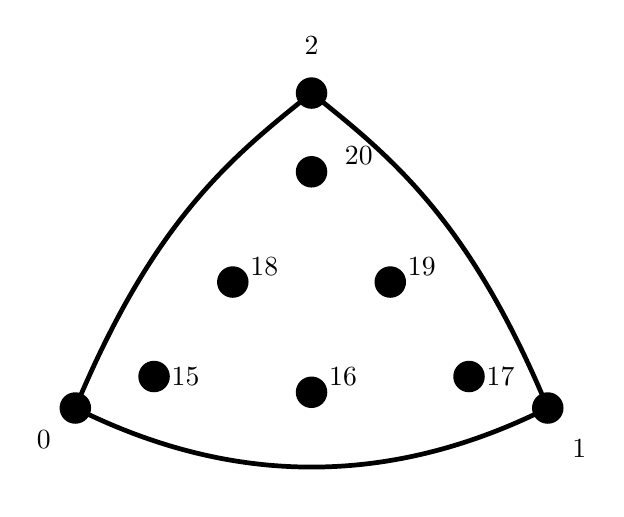
\begin{tikzpicture}[scale=4.0] 
\draw [line width=0.6mm, black ] (0, 0) .. controls (0.5,-0.25) and (1.0, -0.25)
   .. (1.5, 0.) .. controls (1.25,0.6) and (1.0,0.8) 
   .. (0.75,1.) .. controls (0.5,0.8) and (0.25,0.6) 
   .. (0,0); 

\path (-0.1,-0.1) node {$0$}

(1.6,-0.13) node {$1$}

(0.75,1.15) node {$2$}
(0.35,0.1) node {$15$}
(0.85,0.1) node {$16$}
(0.60,0.45) node {$18$}
(1.35,0.1) node {$17$}
(1.1,0.45) node {$19$}
(0.9,0.8) node {$20$};

\fill (0,0) circle [radius=0.5mm];
\fill (1.5,0) circle [radius=0.5mm];
\fill (0.75,1.) circle [radius=0.5mm];
\fill (0.25,0.1) circle [radius=0.5mm];
\fill (0.75,0.05) circle [radius=0.5mm];
\fill (1.25,0.1) circle [radius=0.5mm];
\fill (1.0,0.4) circle [radius=0.5mm];
\fill (0.5,0.4) circle [radius=0.5mm];
\fill (0.75,0.75) circle [radius=0.5mm];
\end{tikzpicture}
\end{figure}
\end{frame}
\begin{frame}{Ordering - Tetrahedron}
The ordering for a tetrahedron is similar to that of a triangle, with vertices, edges, faces, and then internal points. For a cubic tetrahedron (no internal control points), the ordering is as below, based on the canonical vertex, edge, and face ordering for a linear tetrahedron.
{
  \scriptsize

\begin{eqnarray*}
&\;\;\;\;\;\;\;\;\;\;\;\;\;\;\;\;\;\;\mathbf{C}_{3}\;\mathbf{C}_{15}\mathbf{C}_{14}\mathbf{C}_{2}\;&\mathbf{C}_{0003}\mathbf{C}_{0012}\mathbf{C}_{0021}\mathbf{C}_{0030}\\
&\;\;\;\;\;\;\;\;\;\;\;\;\mathbf{C}_{13}\mathbf{C}_{18}\mathbf{C}_{7}\;&\mathbf{C}_{0102}\mathbf{C}_{0111}\mathbf{C}_{0120}\\
&\;\;\;\;\;\;\mathbf{C}_{12}\mathbf{C}_{6}\;&\mathbf{C}_{0201}\mathbf{C}_{0210}\\
&\mathbf{C}_{1}\;&\mathbf{C}_{0300}\\
\\
&\;\;\;\;\;\;\;\;\;\;\;\;\mathbf{C}_{11}\mathbf{C}_{19}\mathbf{C}_{8}\;&\mathbf{C}_{1002}\mathbf{C}_{1011}\mathbf{C}_{1020}\\
&\;\;\;\;\;\;\mathbf{C}_{17}\mathbf{C}_{16}&\mathbf{C}_{1101}\mathbf{C}_{1110}\\
&\mathbf{C}_{5}\;&\mathbf{C}_{1200}\\
\\
&\;\;\;\;\;\;\mathbf{C}_{10}\mathbf{C}_{9}\;&\mathbf{C}_{2001}\mathbf{C}_{2010}\\
&\mathbf{C}_{4}\;&\mathbf{C}_{2100}\\
\\
&\mathbf{C}_{0}\;&\mathbf{C}_{3000}\\
\\
\end{eqnarray*}
}
\end{frame}
\begin{frame}{Aligning Shared Nodes}
When obtaining the nodes for a particular triangle, specific ordering must be considered. This is due to edges not necessarily being oriented with the face. In \texttt{alignSharedNodes}, this problem is addressed by using \texttt{getAlignment} and specifying the order. If an edge is flipped with respect to the triangle, the ordering of the edge nodes is reversed and the correct ordering of nodes for the triangle is obtained.

\end{frame}
\begin{frame}{Aligning Shared Nodes}
Ordering of edge nodes is the same as for a triangle, reversing them if they are flipped relative to the tetrahedron. For the face nodes in the tetrahedron, these can be flipped and rotated. The correct re-ordering is implemented in a more general form, but uses the fact the interior nodes form loops around the vertices, and rotation is just a shift by the number of nodes per edge. Flipped faces are less obvious, but the correct ordering is obtained by simply examining the flipped triangle's nodes, and matching the ordering (in the example below, node 6 is where node 0 is in the canonical triangle, so the ordering starts with 6). Examples are shown below.
\end{frame}
\begin{frame}{Aligning Shared Nodes}
\begin{figure}[!ht]
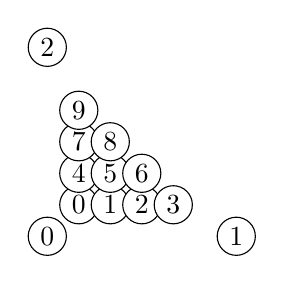
\begin{tikzpicture}[scale=0.4]
\tikzstyle{every node}=[circle, draw, fill=white,
                        inner sep=2pt, minimum width=5pt]
\path (0,0) node {$0$}

(6,0) node {$1$}
(0,6) node {$2$}
(1,1) node {$0$}
(2,1) node {$1$}
(3,1) node {$2$}
(4,1) node {$3$}
(1,2) node {$4$}
(2,2) node {$5$}
(3,2) node {$6$}
(1,3) node {$7$}
(2,3) node {$8$}
(1,4) node {$9$};

\end{tikzpicture}\hspace{0.5cm}
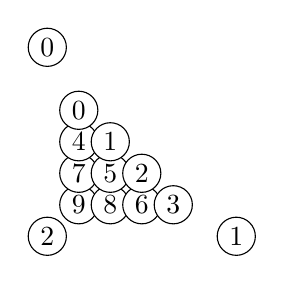
\begin{tikzpicture}[scale=0.4]
\tikzstyle{every node}=[circle, draw, fill=white,
                        inner sep=2pt, minimum width=5pt]
\path (0,0) node {$2$}

(6,0) node {$1$}
(0,6) node {$0$}
(1,1) node {$9$}
(2,1) node {$8$}
(3,1) node {$6$}
(4,1) node {$3$}
(1,2) node {$7$}
(2,2) node {$5$}
(3,2) node {$2$}
(1,3) node {$4$}
(2,3) node {$1$}
(1,4) node {$0$};
\end{tikzpicture}\hspace{0.5cm}
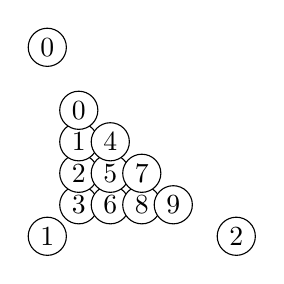
\begin{tikzpicture}[scale=0.4]
\tikzstyle{every node}=[circle, draw, fill=white,
                        inner sep=2pt, minimum width=5pt]
\path (0,0) node {$1$}
(6,0) node {$2$}
(0,6) node {$0$}
(1,1) node {$3$}
(2,1) node {$6$}
(3,1) node {$8$}
(4,1) node {$9$}
(1,2) node {$2$}
(2,2) node {$5$}
(3,2) node {$7$}
(1,3) node {$1$}
(2,3) node {$4$}
(1,4) node {$0$};
\end{tikzpicture}

\end{figure}
The above diagram describes shared nodes for 6th order B{\'e}zier triangle. Original Ordering (left) (0,...,9). Flipped ordering (middle) (9,8,6,3,7,5,2,4,1,0). Rotated ordering by 2 (right) (3,6,8,9,2,5,7,1,4,0). All of this information is in \texttt{crvTables.cc}.
\end{frame}
\begin{frame}{Split Point Locations on Triangles}
This is an implementation detail used for interpolation points.\spa
Given barycentric coordinates $u,v,w=1-u-v$ such that on a triangle in parameter space, $\mathbf{p} = u\mathbf{p}_0 + v\mathbf{p}_1 + w\mathbf{p}_2$ we are interested in splitting it at a given $(u,v,w)$. Due to denegeracy and periodicity, lets define this as a pair of linear splits, such that $ \mathbf{q} = a\mathbf{p}_0 + (1-a)\mathbf{p}_1 $ and $\mathbf{p} = b\mathbf{p}_2 + (1-b)\mathbf{q}$. Solving for $(a,b)$ gives $ a = v/(u+v), b = 1-u-v$. This is implemented in \texttt{crvSnap.cc}.

\end{frame}
\end{document}
